%% 
%% Copyright 2019-2021 Elsevier Ltd
%% 
%% This file is part of the 'CAS Bundle'.
%% --------------------------------------
%% 
%% It may be distributed under the conditions of the LaTeX Project Public
%% License,  either version 1.2 of this license or (at your option) any
%% later version.  The latest version of this license is in
%%    http: //www.latex-project.org/lppl.txt
%% and version 1.2 or later is part of all distributions of LaTeX
%% version 1999/12/01 or later.
%% 
%% The list of all files belonging to the 'CAS Bundle' is
%% given in the file `manifest.txt'.
%% 
%% Template article for cas-sc documentclass for 
%% single column output.

\documentclass[a4paper, fleqn]{cas-sc}

% If the frontmatter runs over more than one page
% use the longmktitle option.

%\documentclass[a4paper, fleqn, longmktitle]{cas-sc}

%\usepackage[numbers]{natbib}
%\usepackage[authoryear]{natbib}
\usepackage[authoryear, longnamesfirst]{natbib}
\usepackage{graphicx}
\usepackage{multirow}
\usepackage[normalem]{ulem}
\useunder{\uline}{\ul}{}
\usepackage{lscape}
\usepackage{longtable}
\usepackage{booktabs, tabularx}
\usepackage{float}
\usepackage{subfigure}
\usepackage{amsthm}
\usepackage{amssymb}
\usepackage{enumitem}
\usepackage[linesnumbered, ruled, vlined]{algorithm2e}
\usepackage[colorlinks]{hyperref}
\usepackage[noabbrev,  nameinlink]{cleveref}

\theoremstyle{definition}
\newtheorem{definition}{Definition}[section]

\theoremstyle{remark}
\newtheorem*{remark}{Remark}

%%%Author macros
\def\tsc#1{\csdef{#1}{\textsc{\lowercase{#1}}\xspace}}
\tsc{WGM}
\tsc{QE}
%%%



% Redefine the label format for equations
\crefformat{equation}{#2Equation~#1#3}
\Crefformat{equation}{#2Equation~#1#3}



% Uncomment and use as if needed
%\newtheorem{theorem}{Theorem}
%\newtheorem{lemma}[theorem]{Lemma}
%\newdefinition{rmk}{Remark}
%\newproof{pf}{Proof}
%\newproof{pot}{Proof of Theorem \ref{thm}}

\begin{document}
\let\WriteBookmarks\relax
\def\floatpagepagefraction{1}
\def\textpagefraction{.001}

% Short title
\shorttitle{MvS CNN-BiLSTM for Urban $PM_{2.5}$ Concentration Prediction of India}    

% Short author
\shortauthors{S. Kumar}  

% Main title of the paper
\title [mode = title]{Multi-view CNN-BiLSTM (MvS CNN-BiLSTM) for Urban $PM_{2.5}$ Concentration Prediction of India's Polluted Cities}  


\begin{comment}
% Title footnote mark
% eg:  \tnotemark[1]
\tnotemark[<tnote number>] 

% Title footnote 1.
% eg:  \tnotetext[1]{Title footnote text}
\tnotetext[<tnote number>]{<tnote text>} 

% First author
%
% Options:  Use if required
% eg:  \author[1, 3]{Author Name}[type=editor, 
%       style=chinese, 
%       auid=000, 
%       bioid=1, 
%       prefix=Sir, 
%       orcid=0000-0000-0000-0000, 
%       facebook=<facebook id>, 
%       twitter=<twitter id>, 
%       linkedin=<linkedin id>, 
%       gplus=<gplus id>]

\author[<aff no>]{Subham Kumar}[<options>]

% Corresponding author indication
\cormark[<corr mark no>]

% Footnote of the first author
\fnmark[<footnote mark no>]

% Email id of the first author
\ead{subh700454@gmail.com}

% URL of the first author
\ead[url]{<URL>}

% Credit authorship
% eg:  \credit{Conceptualization of this study,  Methodology,  Software}
\credit{<Credit authorship details>}

% Address/affiliation
\affiliation[<aff no>]{organization={}, 
            addressline={},  
            city={}, 
%          citysep={},  % Uncomment if no comma needed between city and postcode
            postcode={},  
            state={}, 
            country={}}

\author[<aff no>]{<author name>}[<options>]

% Footnote of the second author
\fnmark[2]

% Email id of the second author
\ead{}

% URL of the second author
\ead[url]{}

% Credit authorship
\credit{}

% Address/affiliation
\affiliation[<aff no>]{organization={}, 
            addressline={},  
            city={}, 
%          citysep={},  % Uncomment if no comma needed between city and postcode
            postcode={},  
            state={}, 
            country={}}

% Corresponding author text
\cortext[1]{Corresponding author}

% Footnote text
\fntext[1]{}

% For a title note without a number/mark
%\nonumnote{}


\end{comment}



% Here goes the abstract
\begin{abstract}
The presence of $PM_{2.5}$ is a major concern for human well-being and ecosystems. The effective measure of $PM_{2.5}$ is the vital problem worldwide. These tiny particles can quickly enter the respiratory system and deeply infiltrate the lungs,  leading to various health issues,  including respiratory disorders,  cardiovascular diseases,  and premature death. The literature shows that hybrid deep learning (DL) models are performing better than stand-alone DL models of time series (i.e., CNN, RNN, GRU, LSTM and BiLSTM) to predict the $PM_{2.5}$ pollutant, but effective performance is not been achieved yet. In this research, the author has proposed a hybrid stacked CNN Bidirectional-LSTM model architecture that utilises the multiple views of the data corresponding to seasonal repetitions to induce the multiple models, called Multi-view Stacked CNN Bidirectional-LSTM (MvS CNN-BiLSTM). The proposed model has been deployed over seventeen univariate time series ($PM_{2.5}$) data of highly polluted Indian cities and stand-alone DL models. The performances of the proposed model have been compared using Root Mean Square Error (RMSE) and Mean Absolute Percentage Error (MAPE) measures. The average enhancement of the proposed model on all datasets has been achieved compared to stand-alone DL models as \textcolor{red}{RMSE:  7.11\% (CNN), 5.08\% (RNN), 3.80\% (GRU), 5.57\% (LSTM) and 4.05\% (BiLSTM) and MAPE: 27.16\% (CNN), 28.52\% (RNN), 26.22\% (GRU), 27.22\% (LSTM), 23.11\% (BiLSTM).} Moreover, the non-parametric statistical analysis (Friedman and Holm\'s) have been performed and proves that the proposed model MvS CNN-BiLSTM is performed as distinct and effective over both performance measures.
\end{abstract}

% Use if graphical abstract is present
%\begin{graphicalabstract}
%\includegraphics{}
%\end{graphicalabstract}
%
%% Research highlights
%\begin{highlights}
%\item 
%\item 
%\item 
%\end{highlights}

% Keywords
% Each keyword is separated by \sep
\begin{keywords}
 \sep Air Pollution \sep  Deep Learning \sep Time Series \sep MultiView \sep $PM_{2.5}$
\end{keywords}

\maketitle

% Main text
\section{Introduction}
Air pollution has become a major global problem due to industrialisation and urbanisation. The rising levels of air pollutants,  such as CO,  SO,  $O_3$,  $PM_{10}$,  and $PM_{2.5}$. It has led to environmental issues like soil acidification,  fog, haze and severe health problems such as heart attacks and lung diseases. The World Health Organization has revealed that contaminated air affects most of the global population,  approximately 90\% (\cite{zhou2019effects}). $PM_{2.5}$,  or 2.5 micrometres or less aerodynamic diameter particulate matter, is an essential factor in calculating the Air Quality Index (AQI). AQI is a numerical scale used to communicate how polluted the air is and its potential health effects to the public. $PM_{2.5}$ is a crucial air pollutant that can infiltrate the respiratory system and have detrimental health consequences. Time series data is a sequential data type collected at regular intervals, with time as the index. It involves examining trends and patterns,  with stationarity important, implying statistical properties' constancy over time. Forecasting based on historical patterns finds widespread applications in various fields,  providing valuable decision-making and predictive modelling insights.

Three principal methods,  namely deterministic,  statistical,  and Machine learning (ML)/Deep Learning(DL),  are widely utilised in predicting air quality. Deterministic methods simulate atmospheric chemistry's dispersion and transport processes,  but they can be computationally expensive and less accurate due to limited actual observations. Statistical methods rely on historical data to forecast pollutant concentrations,  but their linear assumptions may limit prediction performance. Researchers are incorporating non-linear machine learning models to surpass these constraints as alternative methods for predicting air quality. Machine learning and Deep Learning models such as Support Vector Machines (SVM) (\cite{lin2011forecasting}), Autoregressive-Integrated Moving Average (ARIMA) (\cite{kumari2022machine}),  Linear Regression(LR) (\cite{kumari2022deep}),  Artificial Neural Networks (ANNs) (\cite{taylan2017modelling}) and Fuzzy Logic (FL) (\cite{wang2015model}) have been applied in air quality prediction studies. ANNs have been particularly popular among them,  showing promising results in various applications. However,  the rapid development of deep learning techniques has outperformed traditional ML models. Deep learning models,  such as Long Short-Term Memory (LSTM) (\cite{kristiani2022short}),  Gated Recurrent Units (GRU),  and Convolutional Neural Networks (CNN) (\cite{ayturan2018air}),  have shown improved prediction performance by capturing long-term dependencies and spatial features in air quality data.


Multi-view learning (\cite{zhao2017multi, xu2013survey}) has emerged as a potent methodology in machine learning and deep learning. It effectively utilises multiple perspectives or representations of data to enhance predictive performance,  improve generalisation,  and address intricate real-world problems. The technique has garnered significant attention due to its ability to manage varied and complementary information from multiple sources or modalities. This approach holds promise in its application and usability for ML/DL models across different domains,  including Text and Image Analysis (\cite{yang2020image, nie2017auto}),  Audio and Video Processing (\cite{garcia2018multi, hussain2021comprehensive}),  and Environmental Monitoring (\cite{huang2017multi}).

Combining multi-view incorporation and hybrid deep learning models is a powerful technique in modern machine learning. This methodology improves predictive accuracy and feature extraction by integrating different data perspectives and utilising diverse neural network architectures. This approach finds applications in various domains, including sentiment analysis, personalised healthcare diagnostics, and autonomous systems, enhancing performance and providing a deeper understanding of complex datasets.


Given the limited amount of research on anticipating air quality at larger temporal resolutions such as daily or weekly,  which results in lower prediction precision due to fewer samples,  this paper proposes a methodology framework that incorporates bidirectional LSTM neural networks and transfers learning techniques to address this problem and compare its performance to that of conventional machine learning methods.


\section{Review of Literatures}

The authors used different deep learning architectures like GNN-LSTM Fully Connected (FC) network (\cite{li2023nested}),  Wavelet,  ANFIS,  PSO (\cite{pruthi2022low}),  LSTM Deep Feedforward Neural Network (\cite{menares2021forecasting}),  Parallel multi-input 1DCNN-biLSTM (\cite{zhu2023deep}),  LGB algorithm (\cite{kim2022short}),  GOCI-based model,  MAIAC-based model (\cite{lee2021potential}),  MTCAN model (\cite{samal2021multi}),  RNN (\cite{kurnaz2022prediction}),  LSTM16 (\cite{das2022prediction}),  CNN-LSTM (\cite{natsagdorj2023prediction}),  Conv LSTM (\cite{zhu2023deep}),  TL-BLSTM (\cite{ma2019improving}),  CNN+LSTM (\cite{qin2019novel}),  LSTM NN extended (LSTME) (\cite{li2017long}). Autoencoder-based LSTM to predict air pollutant concentrations. They analysed and compared the performance of these models concerning traditional statistical methods and evaluated the impact of exogenous variables on the model's performance. The state-of-art models are compared to their proposed model with traditional DL models.

Despite the advancement,  it is lucid that additional comprehensive and varied datasets are mandatory to refine the acuteness of profound learning models. Certain studies' inability to incorporate exogenous variables limits the models' effectiveness in capturing external factors that could impact air quality. Future studies should tackle these deficiencies and investigate the potential of profound learning models for anticipating different air toxins and meteorological information in various urban improvement situations (\cite{samal2021multi}).

The research studies on air pollution forecasting using various deep learning models conducted by different authors have been summarised in the \Cref{t_lr}. The studies were executed in assorted regions worldwide and at different times. This investigation evaluated function measurements including Root Mean Squared Error (RMSE) (\cite{das2022prediction, kurnaz2022prediction, samal2021multi, kim2022short, zhu2023investigation, menares2021forecasting, nath2021long, du2019deep, li2017long, qin2019novel, ma2019improving, natsagdorj2023prediction}),  Mean Absolute Error (MAE) (\cite{li2023nested, menares2021forecasting, zhu2023investigation, ma2019improving, nath2021long, du2019deep, li2017long}),  Mean Absolute Percentage Error (MAPE) (\cite{li2017long, ma2019improving}),  and R-squared ($R^2$) values (\cite{eren2023predicting, lee2021potential, kim2022short, zhu2023investigation, menares2021forecasting}). Different information sources were utilised,  such as the US EPA (\cite{li2023nested}),  CPCB India (\cite{nath2021long, samal2021multi, pruthi2022low}),  Ministry of the Environment,  Ministry of Environmental Protection,  ground-based observation stations,  and air quality monitoring stations. It can be absorbed that RMSE \& MAPE are the frequently used performance measures.
 
The present study provides a summary (\Cref{t_lr}) of various investigations conducted on air quality based on different data sources employed for their models. These data sources are widely diverse, covering regions such as North America, Delhi (India), Santiago Chile, Shanghai China, Washington US, Sichuan Basin, Beijing (China), and others. The time intervals for data collection employed by these studies varied greatly, ranging from hourly to daily to 15-minute intervals. The data used in these investigations is predominantly collected from environmental monitoring agencies, government agencies, or ground-based observation stations. The broad range of data sources and collection intervals highlights the worldwide scope of air quality research and the plethora of techniques used to collect data.

Moreover,  the analyses have additionally brought to light the potential function of metropolitan woodlands in reducing $PM_{2.5}$ (\cite{kumar2022deep}) concentration. It was found that AOD data could predict $PM_{2.5}$ concentration in resource-limited environments. The computation of air toxin levels affected by the Covid-19 crisis was also studied. Some research has delved into the efficacy of particular deep-learning model pairings in forecasting air pollutant concentrations (\cite{du2019deep}). The investigations have identified areas for improvement in air pollution forecasting,  including enhancing data precision,  considering alternative contaminants,  and integrating dynamic parameters,  as well as addressing issues related to computational cost,  resource intensity,  spatial resolution,  and short-term prediction capability,  with emphasis on the significance of continuous data and the effectiveness of LSTM models in capturing synoptic patterns (\cite{ZHANG2022134890}).

The research gaps vary among the studies, reflecting areas where further investigation or improvement is needed. Some common research gaps include the need to incorporate additional variables or pollutants into the models, explore new data preprocessing techniques, enhance historical data availability, improve model accuracy, and refine the selection of high-resolution variables. Other research gaps involve incorporating more comprehensive meteorological and traffic data, applying deep learning techniques, and addressing the potential for enhancing model performance by including exogenous variables. These research gaps highlight the ongoing efforts to enhance air quality forecasting models and provide valuable insights for future research directions.



\begin{landscape}
  \setlength{\tabcolsep}{3pt}
  
  {\renewcommand{\arraystretch}{1}%
  \begin{longtable}[h!]{ p{0.12\linewidth} p{0.27\linewidth} p{0.16\linewidth} p{0.16\linewidth} p{0.22\linewidth} }%{|l|l|l|l|l|l|}{llllllll}
  \caption{summary of recent state-of-art based on Data,  Model proposed,  Performance measures and Research gap.}
  \label{t_lr}\\
  \hline
  Authors                    & Data                                                                                                     & Performance Measures (RMSE,  MAE, MAPE,  $R^2$)                                                                    & Model                                                               & Research Gap                                                       \\ \hline
  \endhead
  %
  \hline
  \endfoot
  %
  \endlastfoot
  %
  \cite{li2023nested}                & North America (Jan 21 -Sep 21)   Hourly Data collected from US EPA                                       & MAE:  2.81                                                                                               & GNN-LSTM Fully Connected (FC) network                              & Adding more variables and new data preprocessing technique for enhancing model.                                    \\
  \cite{pruthi2022low}           & Delhi  India (18 -21) Daily Data collected from   CPCB India.                                            & Correlation coefficients:  {[}0.96, 0.98{]} (1   day),  {[}0.86, 0.93{]} (2 days),  {[}0.82, 0.91{]} (3 days) & Wavelet,  ANFIS,  PSO                                                 &  Adding more historical data for enhance model.                                                  \\
  \cite{menares2021forecasting}             & Santiago Chile (05 - 19) Hourly   Data provided by Ministry of the Environment                           & RMSE 3.88,  MAE 2.52,  $R^2$ 0.94                                                                            & LSTM Deep Feedforward Neural Network                               & Add more pollutants for enhance the model.               \\
 \cite{zhu2023investigation}            & Shanghai china (2014-05-13 to 2020-12-31)   Hourly Data provided by Ministry of Environmental Protection & RMSE 3.88,  MAE 2.52,  $R^2$ 0.94                                                                            & Parallel multi-input 1D-CNN-biLSTM   model                          & add  factory data ,  creating a Smartphone Application for PM2.5 forecasting.                                                         \\



 \cite{MANDAL2023137036} & Delhi India (1 Jan 2018- 30 Nov 2019) 15 min interval data collected from CPCB Inda. &$R^2=0.75$,  $RMSE=25.13$,  $MAE: 21.28$ & Cluster-based Graph Neural Network (SA-GNN) & Add activation function, add more historical data \\
 \cite{MA2019117729} & Washington, US (1st January to 31st January 2017) hourly data collected from US (EPA) & $RMSE = 0.043$ & Geo-LSTM & Add more Data with more futures of Data.  \\
 \cite{ZHANG2022134890}& Sichuan Basin (January 1,  2019,  to December 31,  2019) Hourly data collected from  China Environmental Monitoring Center  & $R^2= 0.917$, $RMSE=7.4$ & data-driven spatial autocorrelation terms (DDW-RF) & necessary to select more appropriate high-resolution variables. \\
\cite{TIAN2022134048} & Beijing,  Tianjin,  Dalian,  and Yantai (1600 hour) China & $MAPE=6.0819$, $RMSE=11.8654$, $R^2=0.9754$ &  multi-objective optimisation algorithm & Add more pollutants, improving accuracy \\
\cite{DAI2022131898} &shaanxi province ( January 1,  2016, to December 31,  2020 ) daily data & $RMSE=0.3997$, $MAPE=0.14599$, $MAE=0.2871$ &GBoost-MLP based on GARCH model & apply deep learning model \\ 
\cite{AGGARWAL2021129660} & India (January 2016 to December 2018) 15-minute interval  & $RMSE=19.89, 25.88$ ,  $R^2=0.96, 0.9$ &lstm&apply more pollutants \\

 \cite{kim2022short}         & Seoul South Korea ( July 2018 to   June 2021) Deliy Data                                                 & bias = -0.25\% to -0.10\%,  RMSE =   32.45\%-33.23\%,  $R^2$ = 0.83-0.86                                     & LGB algorithm                                                       & Add more data for enhance the model.                                                                            \\





  \cite{lee2021potential}            & Seoul Korea (16 -19) Hourly Data collected from ground-based observation stations                      & $R^2$ values:  0.61 and 0.78                                                                                & GOCI-based model, MAIAC-based model                                & Add more pollutants and Data for enhance the model.                                                                   \\




 \cite{samal2021multi}  & Talcher India (02/02/2018 to   04/07/2020) per 15 min Data collected from CPCB india.                    & RMSE values:  93\%  and 90\% better than GRU                                                              & MTCAN model                                                         & add meteorological factors and traffic data for the enhanced model.                                                               \\


 \cite{kurnaz2022prediction}          & Sakarya Urbanization (   01.08.2018 and 31.07.2020) Daliy Data provided from e Ministry of Environment   & RMSE:  2.84–14.09                                                                                       & RNN                                                                 & Add more pollutants and Data for enhance model.    \\



 \cite{das2022prediction}           & Istanbul Basaksehir (01.01.2021   and 09.02.2022) Hourly data taken from Ministry of Environment         & RMSE: 10.229478                                                                                          & LSTM16                                                              & add more pollutants and  meteorological Data for enhance model. data.                                          \\
\cite{natsagdorj2023prediction}              & Ulaanbaatar Mongolia  (June 1,  2018, to  April 30,  2020) Hourly Data from U.S.   Embassy in Mongolia      & RMSE: 11.77                                                                                              & CNN-LSTM                                                            & Add more Data and atmospheric Data for enhance the model.  \\
 \cite{eren2023predicting}         & Istanbul (15-19) Hourly Data collected from Kathane air quality monitoring station                     & $R^2$:  0.98                                                                                               & LSTM+LSTM                                                           & Add more pollutants and Data for enhance the model.           \\




\cite{zhu2023deep}           & Italian city ( March 2004 to   February 2005 ) Hourly Data collected from Kaggle & 91\% Prediction accuracy & Conv.LSTM                                                           & Deploy deep leading models for classification.  \\
 \cite{ma2019improving}               & Guangdong China (3 years) Hourly   Data collected from Guangdong province.                               & RMSE: 8.652,  MAE: 6.184,    MAPE: 27.909                                                                   & TL-BLSTM                                                            & utilising transfer learning techniques and adding more data to enhance the model.     \\
\cite{qin2019novel}       & Shanghi (2015-2017) Daliy Data collected   manually  & RMSE:  14.3   & CNN+LSTM     &  Add more data for enhance model. \\
 \cite{li2017long}          & Beijing China (Jan 2014 -may   2016) Hourly Data collected from Ministry of environmental protection.    & RMSE: 12.6,  MAE: 5.46,  MAPE:  11.93                                                                        & LSTM NN extended(LSTME)                                             & Adding more pollutants to enhance the model.                                           \\
 \cite{du2019deep}         & Beijing China (   01/01/2010-01/31/2010) Hourly Data collected from0 uci.                                 & RMSE: 77.38,  MAE: 54.58                                                                                   & Deep Air Quality Forecasting   Using Hybrid Deep Learning Framework & Add more Data for model enhancing.\\
\cite{nath2021long}       & Kolkata India (Jan 16 - Feb 20)  Daily Data collected from CPCB   India.                               & RMSE: 18.8,  MAE: 15.88                                                                                    & Autoencoder based LSTM                                             &  include exogenous variables for enhance the model. \\ \hline
  \end{longtable}}
  \end{landscape}

  

\section{Material and Method}
In this section of our research,  we will delve into the methodology of predicting $PM_{2.5}$ using various deep-learning models. Our data was obtained from the CPCB\textcolor{red}{(India)} hourly univariate data collection. It focused on a single future $PM_{2.5}$ in this dataset. Then we processed the obtained data and implemented several deep-learning models to generate our forecasts. The primary objective of employing these is to enhance the model's accuracy of our predictions. Our first step was to collect the CPCB hourly univariate data. Then isolated, the data points related to $PM_{2.5}$ for study.
% Figure
\begin{figure*}[h!]
	\centering
		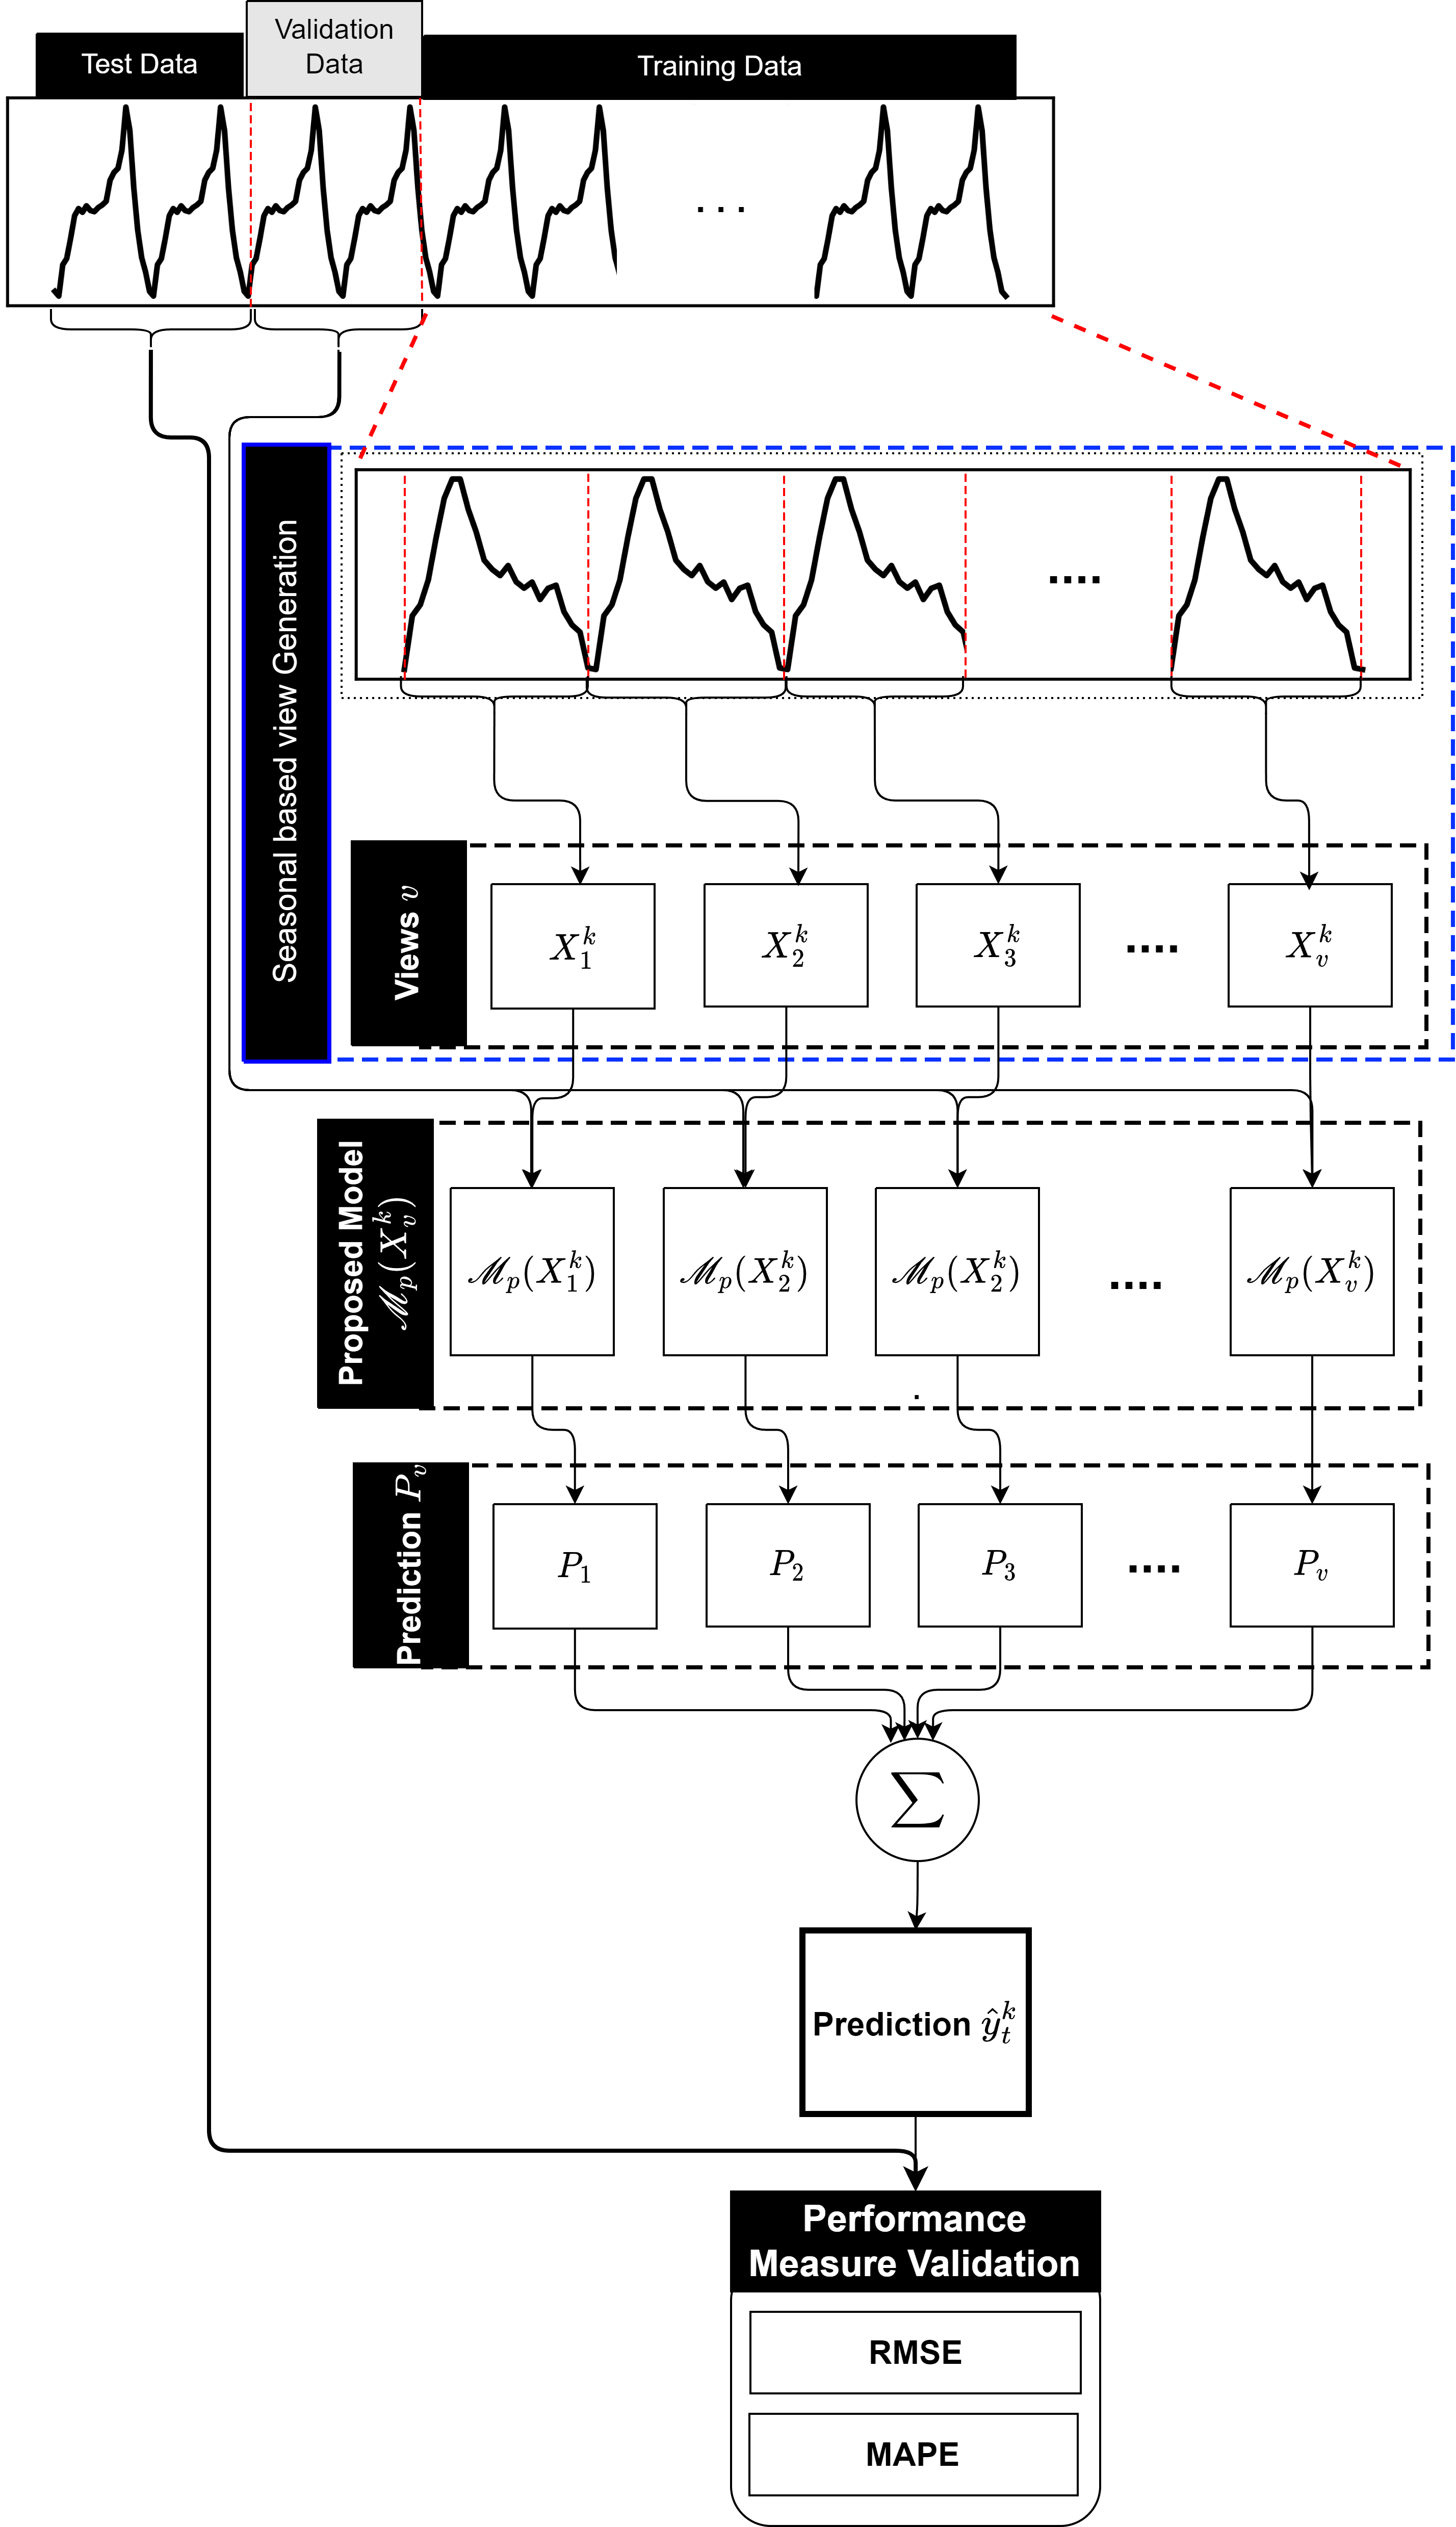
\includegraphics[scale=0.6]{MvS CNN-BiLSTM}
	  \caption{Flow diagram of proposed MultiView Stacked CNN-BiLSTM (MvS CNN-BiLSTM)}\label{Muticbilstm}
\end{figure*}


\subsection{Data: }

\begin{table*}[h!]
  \caption{Statistical exploratory data analyses $($EDA$)$ of 17 Time Series Datasets of polluted Indian cities based on $PM_{2.5}$ (\cite{bhawan2020central}).}
  \label{Eda1}
  
  \begin{tabular}{llccccccccc}
  \hline
  
  D.No. & DataSets & Year  & Samples &Mean &Std & Min &25\% &50\% &75\% & Max\\ \hline
  
 D1 &  BHIWADI          & 2017-2022  & 43394   & 108.03 & 79.76  & 0.02 & 55.22   & 97.32       & 135.36 & 999.99 \\ 
 D2 &  JODHPUR     & 2015-2022 &\textbf{61409} & 84.31 & 56.18 & 0.18 & 53.25   & 84.31 & 93.42   & 999.99 \\
 D3 &  SINGRAULI    & 2017-2022 & 43695   & 84.08 & 78.33 & 0.25 & 32.25   & 66          & 111.25  & 985    \\
 D4 &  ANKLESHWAR   & 2019-2022  & 33535     & 58.47 & 35.83 & 0.51 & 32.75   & 58.47 & 72.24   & 977.39 \\ 
 D5 &  LUDHIANA        & 2017-2022  & 49010  & 54.18 & 41.73 & 0.07 & 29.7    & 47.66       & 64.88   & 999.99 \\
 D6 &  DURGAPUR       & 2020-2022 & \textbf{17434}   & 71.67 & 46.20 & 0.33 & 37.47 & 62.05      & 98.03 & 565.41 \\ 
 D7 &  YAMUNA\_NAGAR  & 2019-2022 & 34299   & 77.86  & 52.31 & 0.1  & 43.8    & 69.91       & 94.28   & 930    \\
 D8 &  CHARKHI\_DADRI  & 2020-2022  & 24099   & 80.19 & 62.81 & 0.01 & 39.54  & 77.92       & 94.49  & 995.1  \\ 
 D9 &  JIND             & 2019-2022 & 34145 & 81.21 & 71.20 & 0.2  & 38.99   & 61.45       & 98.25   & 845.6  \\ 
 D10 &  KURUKSHETRA    & 2019-2022  & 34208 & 68.75& 53.80 & 0.46 & 33.33   & 56.38       & 87.56   & 962.7  \\ 
 D11 &  SONIPAT        & 2019-2022  & 34362  & 54.88 & 43.21  & 0.02 & 27.87   & 49.4        & 62.72   & 543.1  \\ 
 D12 &  DHARUHERA     & 2019-2022 & 34265 & 78.86 & 59.21 & 0.02 & 40.9    & 70.32       & 92.85   & 838.9  \\
 D13 &  AMBALA         & 2019-2022 & 34174 & 61.58 & 45.39 & 0.02 & 32.94   & 51.27       & 76.18 & 754.89 \\
 D14 &  HISAR          & 2019-2022 & 34143 & 86.22 & 71.02 & 0.63 & 42.62   & 69.33       & 102.89 & 999.99 \\ 
 D15 &  FATEHABAD      & 2019-2022 & 34160 & 63.01 & 60.46 & 0.07 & 32.63   & 49.01       & 72.5    & 999.99 \\
 D16 &  BULANDSHAHR  & 2018-2022 & 39869  & 90.53 & 85.08 & 0.25 & 34      & 63.75       & 120.25  & 985    \\ 
 D17 &  MUZAFFARNAGAR  & 2018-2022 & 38786 & 89.29 & 72.84  & 1    & 42.75   & 81.25       & 102.25  & 986    \\ \hline
  \end{tabular}
  \end{table*}
  
The Dataset in this study was collected from the Indian government portal CPCB (Central Pollution Control Board). These datasets contain univariate Time series hourly data of 17 Indian cities,  with most cities providing approximately four years (see in \Cref{Eda1}). The table lists Bhiwadi,  Jodhpur,  Singrauli,  Ankleshwar,  Ludhiana,  Durgapur,  Yamuna Nagar,  Charkhi Dadri,  Jind,  Kurukshetra,  Sonipat,  Dharuhera,  Ambala,  Hisar,  Fatehabad,  Bulandshahr,  and Muzaffarnagar as the 17 cities from which data was collected shown on ( \Cref{India map}) with Name,  Latitude and Longitude. The \Cref{Eda1} also provides information about the number of data points available in datasets, the highest number of data points in Jodhpur, and the lowest number of data points in Durgapur.

In \Cref{Eda1}, All the datasets are thoroughly analysed based on several components such as Count, Min,  Mean,  Std,   25\%, Max,  75\%,  and 50\%. The detailed description of the analysis is then summarised for ease of understanding.
% Figure
\begin{figure*}[h!]
	\centering
		\includegraphics[scale=0.3]{india_map}
	  \caption{Geographical representation of polluted cities of India with their Latitude,  Longitude and Name. }\label{India map}
\end{figure*}


\begin{itemize}

\item
\textbf{Preproccessing:  }
Data preprocessing is critical in machine learning projects as it ensures the data is clean,  consistent,  and ready for analysis. Techniques like missing value imputation and min-max scaling facilitate data normalisation and improve the effectiveness of machine learning algorithms by allowing them to learn from the data and make accurate predictions.
During the initial data preprocessing stage,  missing values are replaced with the means. The dataset is divided into ten parts or chunks,  and the mean is calculated for each chunk. Subsequently,  the means of all the chunks are averaged together,  as shown in.
\begin{equation} \label{equ: mean}
        x_i=\frac{\sum_{i=1}^{k} \left(\frac{D_{c_{i}}}{D_{s_{i}}} \right)}{k}
\end{equation}
 where $k=10$ \& $x_i$ is missing value in time series and $D_c$ represent chanks of Dataset. $D_s$ is the number of available samples in the dataset chunks represented by $D_c$. \\
Once the missing values have been attributed in the dataset using \Cref{equ: mean}, the next step is to apply min-max scaling \Cref{equ: minmax}. This technique ensures that univariate data is scaled to fall within the range of [0, 1]. The scaling is achieved \Cref{equ: minmax}: 
\begin{equation}
        x_{norm,  i}=\frac{x_i - \mu}{max(x)-min(x)}
        \label{equ: minmax}
    \end{equation}
Where $x_i$ is the $i^{th}$ data point and \textcolor{red}{$\mu$} is the mean of univariate data $min(x)$  and $max(x)$ denote the minimum values and maximum values in the univariate series.

Consistency is essential for comparing data across different datasets. Additionally,  the scaling technique reduces the influence of outliers and enhances the data's robustness.


\item
\textbf{Decomposition and analysis: }

In \Cref{Eda}, all subplot has been plotted on 480 Recent data points. \Cref{Eda} presents the graphical representation of the dataset,  showcasing different categories like trend \&  seasonal. In rows 1,  4,  and 7,  the data is labelled as "Original." Rows 2,  5,  and 8 correspond to the "Seasonal" category,  while rows 3,  6,  and 9 represent the "Trend" category. The last \textcolor{red}{two} row combines all three categories,  displaying "Original, " "Seasonal, " and "Trend" data in a single dataset. Each subplot within the graph has a specific dataset name,  indicated in the legend.

The graph consists of five columns,  each corresponding to a specific range of rows (1 to 3,  3 to 6 and 6 to 9) from the dataset. The border colour remains consistent across these columns,  indicating they belong to the same dataset. The legend provides clarity by associating the dataset name with its respective subplot,  facilitating a comprehensive understanding of the data distribution and categories.


\begin{figure*}[h!]
  \centering
  \subfigure{\includegraphics[scale=0.208]{eda1}}
  \subfigure{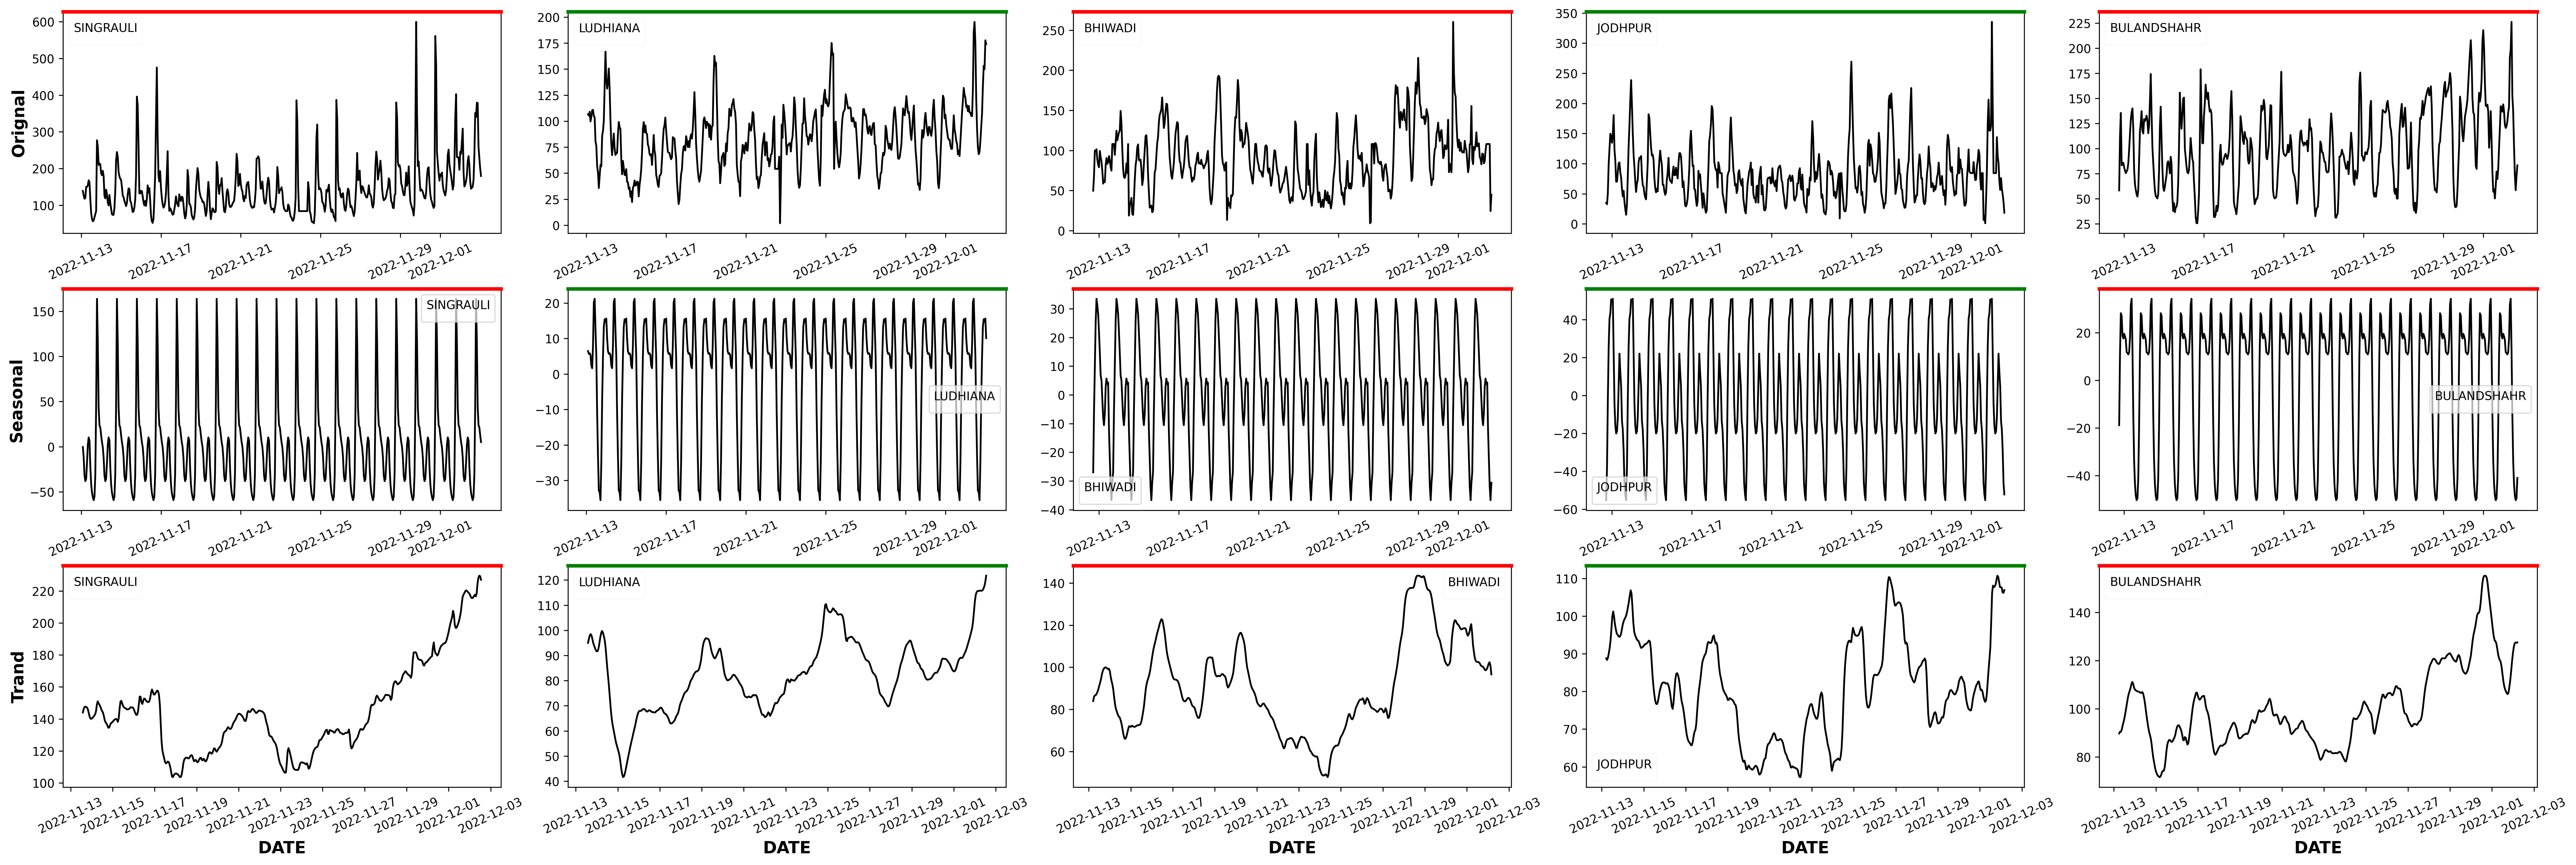
\includegraphics[scale=0.208]{eda2}}
  \subfigure{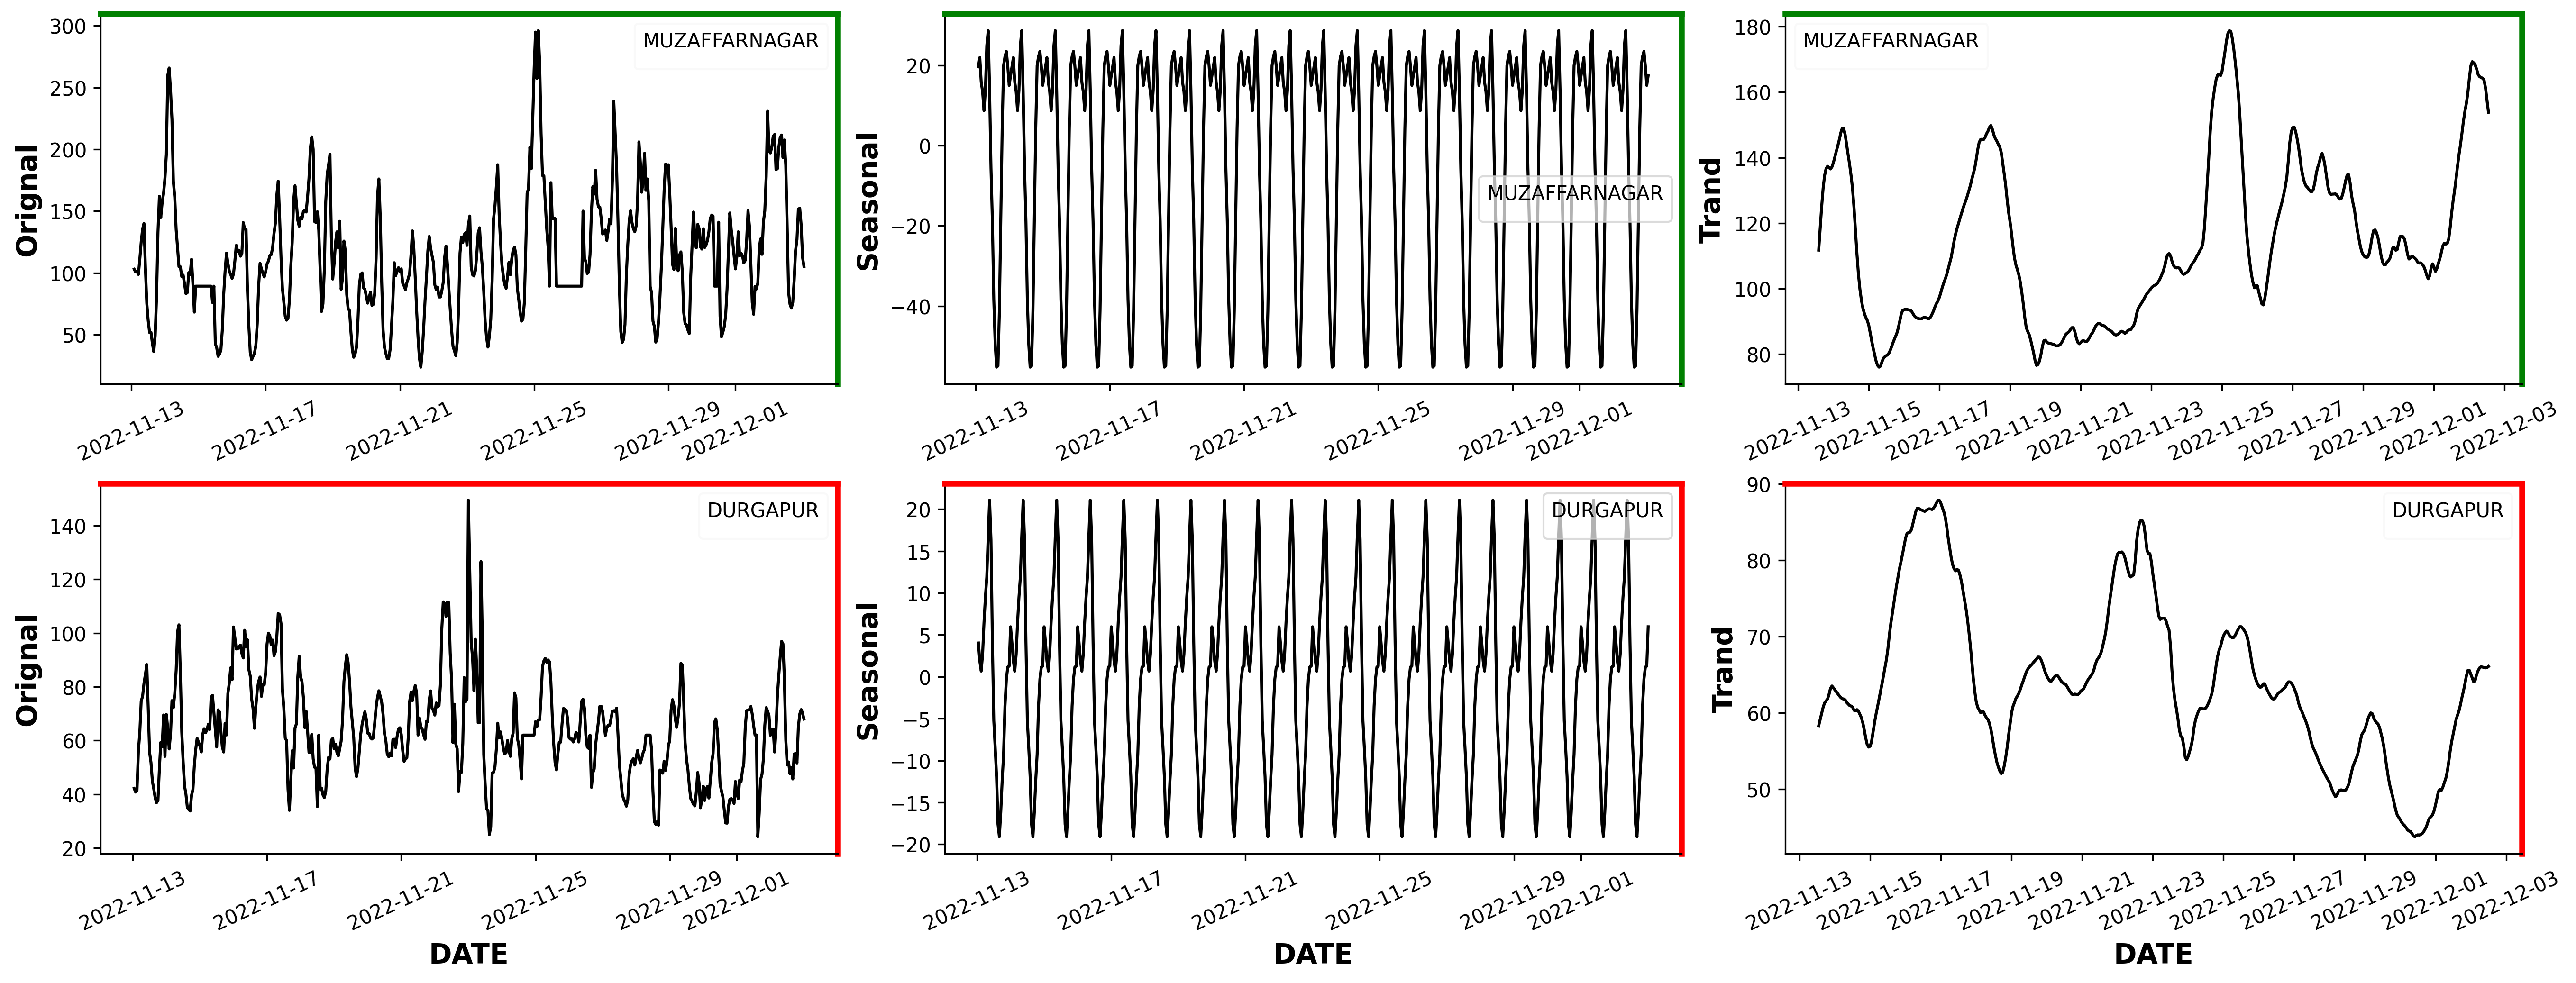
\includegraphics[scale=0.208]{eda3}}
  \caption{Decomposition of 17 data sets based on trend, seasonal, and original dataset.}
  \label{Eda}
\end{figure*}
\Cref{Eda} illustrates the seasonal variations in the dataset with a frequency of every 24 hours. Each subplot within the graph contains 20 data points representing the seasonal pattern. Additionally,  the graph showcases various types of trends present in the data. These trends may include upward, downward,  or fluctuating trends over time. The combination of seasonal variations and diverse trends provides valuable insights into the underlying patterns and behaviours of the dataset.
\end{itemize}

\subsection{Deep learning models}
\subsubsection{Convolutional Neural Network (CNN)}
A CNN is an essential neural network utilised extensively for analysing time series and processing signals. Unlike standard fully connected neural networks,  which process input as vectors,  1D CNNs extract local features using convolution operations using a sliding window technique. They're made to operate with one-dimensional signals like audio or time series sensor readings. In \Cref{CNN} (\cite{chaerun2021comparative}) 1D CNN,  multiple filters are employed to extract various features from the input signal. These filters slide over the input,  capturing local patterns and representations. The convolutional layer output is then downsampled using pooling layers,  reducing the data dimension and preventing overfitting. The network may also include fully connected layers that perform tasks like classification or regression using the retrieved features.

The simplicity of the 1D CNN (\cite{kiranyaz20211d}) architecture lies in its effectiveness in extracting features from one-dimensional signals. The sliding window approach allows the network to focus on local details and extract relevant information effectively. Furthermore,  the convolutional process reduces the number of parameters,  resulting in a more computationally efficient network. Pooling layers help in generalisation by decreasing output complexity,  resulting in higher performance on previously unknown data. 1D CNNs are versatile and practical in various domains since they can examine historical data and extract relevant characteristics. They've shown to be incredibly effective in applications such as speech recognition (\cite{rusnac2022cnn, wang2019end}),  audio categorisation (\cite{ashraf2022role, hu2020device}),  and sensor data processing (\cite{kattenborn2021review, sun2019classification}). Overall,  1D CNNs are potent tools for collecting features from one-dimensional data,  providing essential insights,  and paving the way for signal processing and time series analysis advances.

\begin{figure*}[h!]
  \centering
    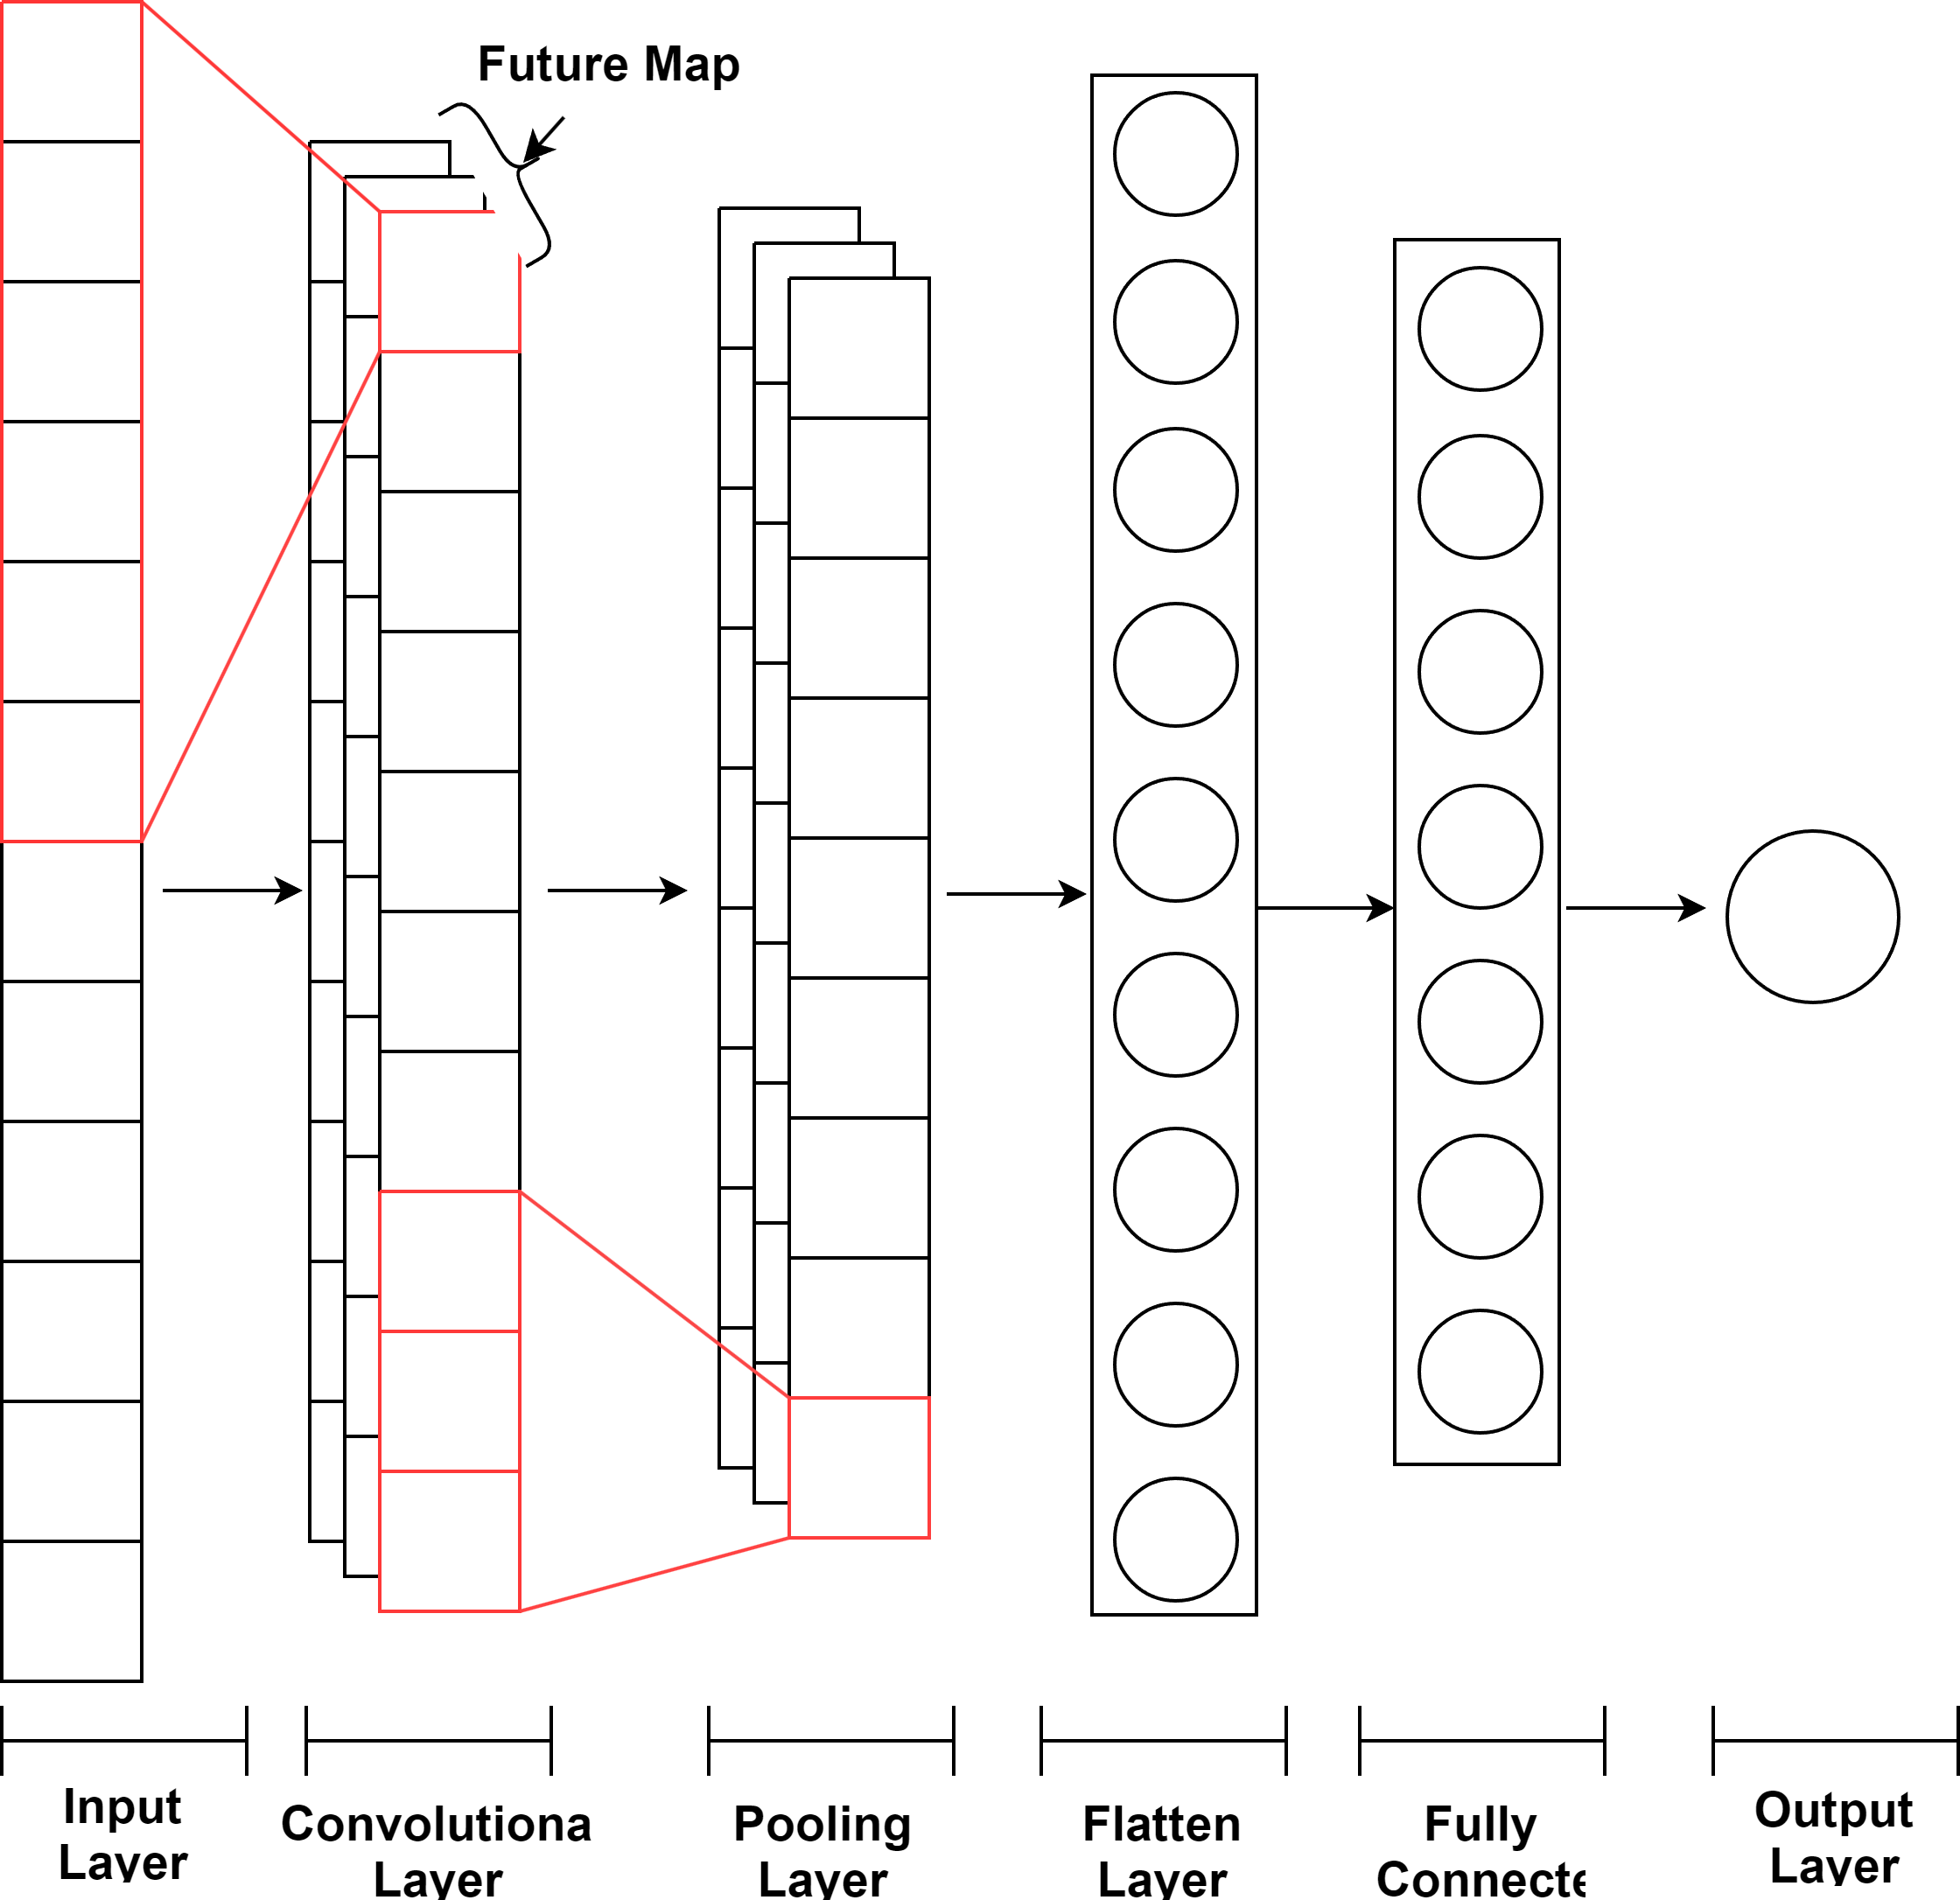
\includegraphics[scale=.5]{cnn}
    \caption{Traditional architecture of $1D-CNN$}\label{CNN}
\end{figure*}

1D CNN uses a set of learnable filters (or kernels) of length k to conduct the convolution operation. This operation involves computing the dot product between the filter and a k-length window sliding over the input sequence x with length L. Then a new sequence of feature maps is generated as an outcome.

Denoting the set of filters as $F$ and the output feature map at position $i$ as $h_i$,  we can express the output feature map $h$ as follows: 
\begin{equation}\label{equ: cnn}
        h_i = \sigma \left (\sum_{j=1}^{k}F_{j}.x_{i+j-1}+b \right)
\end{equation}
Where $F_j$ represents the $j^{th}$ filter in the set of filters $F$,  $x_{i+j-1}$ is the value of the input sequence $x$ at position $(i+j-1)$,  $\sigma$ is the activation function (such as \textcolor{red}{ReLU} or sigmoid),  and $b$ is the bias term.

\subsubsection{Gated Recurrent Unit (GRU)}
The GRU is a specialised recurrent neural network architecture designed for managing sequential data input  (\cite{chung2014empirical}), and the unique proposal was put forth as a substitute for the well-liked LSTM network. These gating mechanisms selectively update the hidden state,  allowing GRU to capture dependencies in sequential data effectively. GRU has found use in an array of areas,  including speech recognition (\cite{shewalkar2019performance, yuan2018auxiliary}),  natural language processing (\cite{cascianelli2018full, wang2020feature}),  and picture recognition (\cite{subramanian2022integrated}),  due to its gating mechanisms and ability to handle sequential dependencies. Its capabilities make it a powerful tool for modelling and understanding sequential data,  providing valuable insights and improved performance in numerous tasks. GRU network based on gates and states are shown in \Cref{up Gru} to \Cref{hid gru}: \\

 
\begin{equation} \label{up Gru}
  Update Gate :  z_t= \sigma(W_{z}\cdot \left[ h_{t-1}, x_t \right]+b_z )
\end{equation}

\begin{equation}\label{r gru}
  Reset Gate :  r_t=\sigma (W_{r}\cdot \left[ h_{t-1}, x_t \right]+b_r )
\end{equation}

\begin{equation} \label{can gru}
  Candidate activation :  \tilde{h_t}=tanh(W_h \cdot \left[ r_t \odot h_{t-1}, x_t \right]+b_h)
\end{equation}

\begin{equation} \label{hid gru}
  Hidden State :   h_t=(1-z_t) \odot h_{t-1}+z_t \odot \tilde{h_t}
\end{equation}



where,  time step t,  the hidden state is represented by $ h_t $,  the input is represented by $ x_t $,  and the update and reset gates are
represented by $ x_t $ and $ r_t$ respectively. The refresh entryway directs the amount of the past covered state to keep for the present time step,  while the reset entryway controls the amount of the past covered state to overlook. The candidate activation $\tilde{h_t}$ represents new information that could be added to the hidden state. The sigmoid activation function $ \sigma $ and element-wise multiplication represented by $\odot$ are used.Weight matrices $ W_z $,  $ W_r $,  $ W_h $ and bias vectors $ b_z $,  $ b_r $,  $ b_h $ are also utilized. The GRU's update and reset gates allow it to learn when to update the hidden state and what information to forget,  making it particularly useful for modelling sequential data with long-range dependencies.
\subsubsection{Recurrent Neural Network (RNN)}
RNN is an ANN that utilises the outcome of the preceding measure to contribute to the present step. Forecasting the succeeding phrase in a statement is not a strong suit of RNNs because their Memory State,  also recognised as the hidden layer,  does not preserve any data about preceding words. It stores the previous input given to the network,  which goes a long way in ensuring accurate predictions. The RNN technique employs identical parameters for every input,  leading to it executing the same function on every hidden layer to obtain the results. Unlike other neural networks, it significantly reduces the complexity of parameters,  making it a popular choice among researchers and developers. The elegance of RNN rests in its capacity to recall prior inputs,  rendering it a valuable instrument in creating predictions that demand context. Ordinarily,  profound learning has been exhibited to be a game-changer in AI and ML,  and it will undoubtedly persist in being an essential instrument in the coming years.

Recurrent Neural Network (RNN) model are input \& output to hidden state can be written as \Cref{equ: ih rnn} \& \Cref{equ: h rnn} respectiveely: 

  \begin{equation} \label{equ: ih rnn}
    Input to Hidden State:  h_t= \psi (W_{hx} \cdot x_t + W_{hh} \cdot h_{t-1} +b_h)
  \end{equation}
  \begin{equation} \label{equ: h rnn}
    Hidden State to Output:  y_t=W_{yh}\cdot h_t+b_y
  \end{equation}
where $h_t $ is the hidden state at time step $t$,  $x_t$ is input at $t$ step of time,  $y_t$ is output at t step of time,  $W_{hx} $ is a weight matrix that links the input to the concealed state,  $W_{hh}$ is the weighted matrix that connects the state that is hidden at time step $t-1$ with the hidden value step t,  $W_{yh}$ is a weighted matrix that links the state that is hidden to the output,  $b_h$ and $b_y$ are biassed terms for both the state that is hidden and the output and $\psi (\cdot)$ is a function of activation applied to the concealed state element by element.


\subsubsection{Long-Short-Term Memory (LSTM)}
LSTMs are a specialised type of RNN designed to handle sequential data. They excel at learning long-term dependencies,  making them suitable for language translation,  speech recognition,  and time series forecasting. Utilising the memory cell and three gates facilitates the capability of LSTMs to learn intricate patterns in data by selectively retaining and discarding information. Deep LSTM networks,  achieved by stacking LSTMs,  are beneficial for tasks like speech recognition (\cite{soltau2016neural, jo2020approximate}) and natural language processing (\cite{wang2015learning, nammous2019natural}). Hochreiter and Schmidhuber  (\cite{hochreiter1997long}) developed LSTMs to overcome the long-term dependency issue in traditional RNNs. LSTMs are widely used in processing (\cite{sahin2018nonuniformly}),  prediction (\cite{gers2000learning}),  and classification (\cite{zhou2015c, karim2017lstm}) of temporal data,  and when combined with CNNs,  they efficiently analyse images (\cite{li2019cnn, rajendran2020land, islam2020combined}) and videos (\cite{ullah2017action, li2020classifying, gao2017video, bin2018describing}) by extracting spatial and temporal features. LSTMs are an effective instrument for analysing sequential data and can be incorporated with other neural network structures to accomplish more complex objectives.
The LSTM architecture-related gates and states are shown in \Cref{lstm i} to \Cref{lstm h}.

  \begin{equation} \label{lstm i}
    Input Gate :  i_t=\sigma (W_{xi}\cdot x_t+W_{hi}\cdot h_{t-1}+b_i)
  \end{equation}
 
  \begin{equation}\label{lstm f}
    Forget Gate :  f_t= \sigma(W_{xf}\cdot x_t +W_{hf}\cdot h_{t-1}+b_f)
  \end{equation}

  \begin{equation}\label{lstm c}
    Candidate Hidden State :   g_t=than(W_{xg}\cdot x_t+W_{hg}\cdot h_{t-1} +b_g)
  \end{equation}

  \begin{equation}\label{lstm ce}
    Cell State :  C_t=f_t \odot C_{t-1}+i_t \odot g_t
  \end{equation}

  \begin{equation}\label{lstm o}
    Output Gate :  o_\sigma(W_{xo}\cdot x_t +W_{ho}\cdot h_{t-1}+b_o)
  \end{equation}

  \begin{equation} \label{lstm h}
    Hidden State :   h_t=o_t \odot tanh(C_t)
  \end{equation}
whare,  $h_t$ at a time step,  is the concealed condition (also known as a hidden representation),  $x_t$  is the time step input,  $C_t$  is the condition of the cell at time step $t$,  serving as the LSTM's long-term memory,  $\sigma$ Its sigmoid activation function,  The tangent hyperbolic activation function is denoted by tanh,  $\odot$ represents element-by-element multiplication,  $W_{xi}$,  $W_{hi}$,  $W_{xj}$,  $W_{hf}$,  $W_{xg}$,  $W_{hg}$,  $W_{xo}$,  $W_{ho}$ are the matrices of that will be taught throughout training and $b_i$,  $b_f$,  $b_g$,  $b_o$ are slanted terms.


\subsubsection{Bi-directional Long Short Term Memory (BiLSTM)}
BiLSTM is a type of human stupidity designed to process sequential data in neither forward nor backward directions. The plan uses dual LSTM layers for forward and backward processing concurrently,  enabling it to grasp the context from previous and upcoming time steps. Therefore,  the network cannot identify any relationships in either direction,  making it a disadvantage for speech recognition and language translation tasks. By providing a broader perspective of the input sequence,  BiLSTMs can improve the performance in tasks requiring contextual understanding. These forms are remarkable for long-term dependencies and are commonly utilised in profound learning projects.

\begin{figure*}[h!]
  \centering
  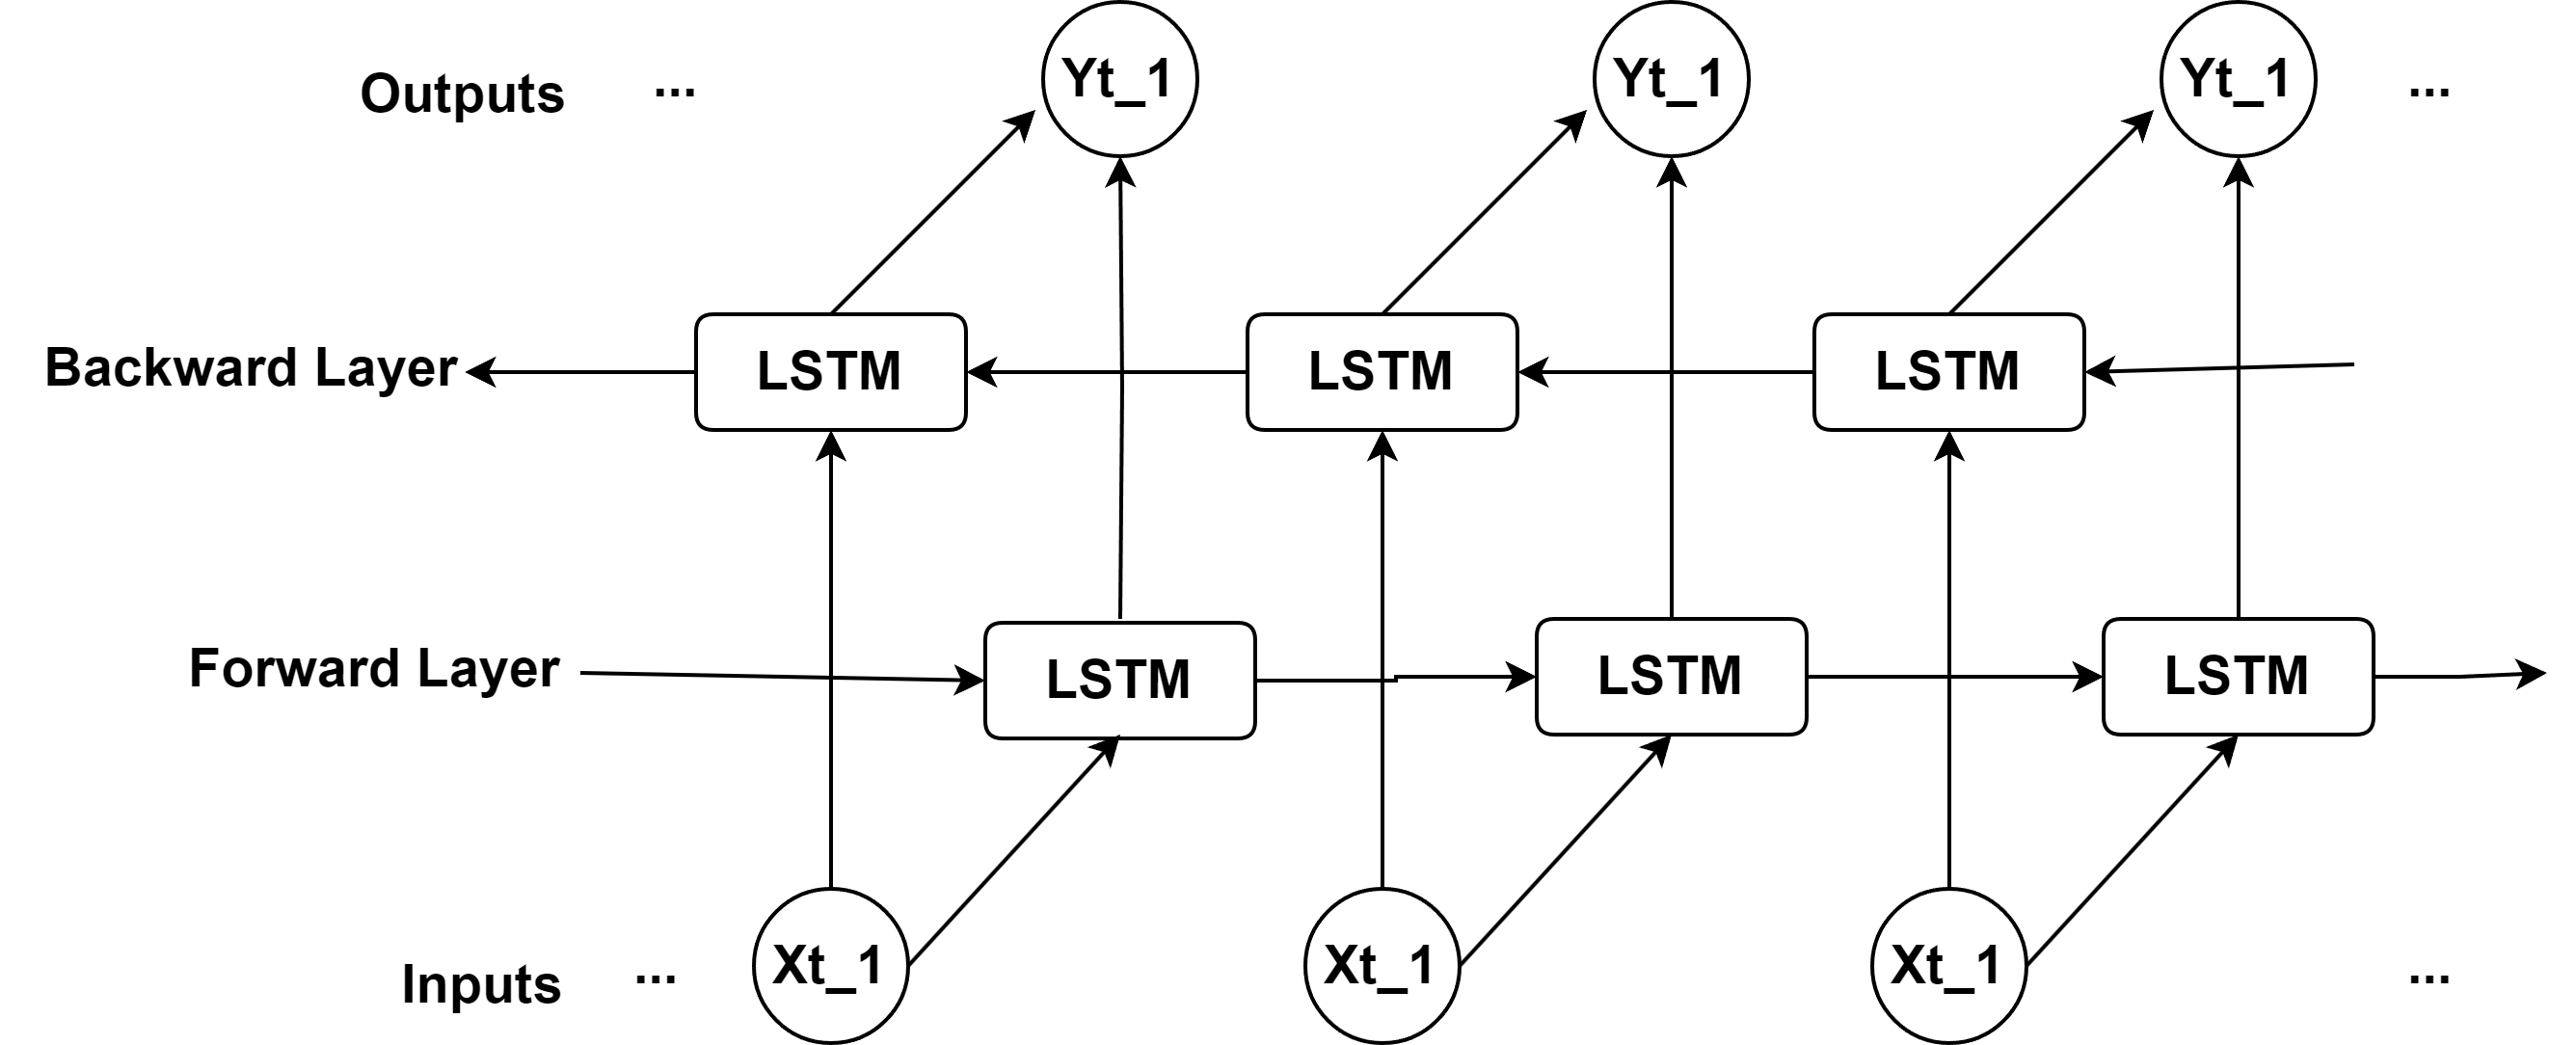
\includegraphics[scale=0.6]{Bilstm}
  \caption{Architecture of BiLSTM (\cite{article})} \label{Bilstm}
\end{figure*}



BiLSTM network architecture gates and states are shown below from \Cref{bi i} to \Cref{bi h}.
\begin{itemize}
  \item  Forward LSTM: \\

    \begin{equation} \label{bi i}
      Input Gate :  i_t^f = \sigma(W_{xi}^f \cdot x_t + W_{hi}^f \cdot h_{t-1}^f + W_{ci}^f \cdot c_{t-1}^f + b_i^f)
    \end{equation}

    \begin{equation}
      Forget Gate :  f_t^f = \sigma(W_{xf}^f \cdot x_t + W_{hf}^f \cdot h_{t-1}^f + W_{cf}^f \cdot c_{t-1}^f + b_f^f) 
    \end{equation}

    \begin{equation}
      Candidate Hidden State :   g_t^f = \text{tanh}(W_{xg}^f \cdot x_t + W_{hg}^f \cdot h_{t-1}^f + b_g^f)
    \end{equation}

    \begin{equation}
      Cell State :  c_t^f = f_t^f \odot c_{t-1}^f + i_t^f \odot g_t^f
    \end{equation}

    \begin{equation}
      Output Gate :  o_t^f = \sigma(W_{xo}^f \cdot x_t + W_{ho}^f \cdot h_{t-1}^f + W_{co}^f \cdot c_t^f + b_o^f)
    \end{equation}

    \begin{equation} \label{bi h}
      Hidden State :   h_t^f = o_t^f \odot \text{tanh}(c_t^f) 
    \end{equation}

  \item Backward LSTM: 
  The formulas for the rear LSTM are similar to those of the forward LSTM but with different weights and biases. The \textcolor{red}{superscript} "b" is used to denote the backward direction (e.g.,  \(W_{xi}^b\) is the weight matrix for the input gate in the backward LSTM). The BiLSTM combines the hidden forward and backwards states to form the final output. The output \(y_t\) at time step \(t\) is typically computed using a combination of both forward and backwards hidden states. The approach for combining the two directions (e.g.,  concatenation,  addition,  etc.) depends on the specific task and model architecture.
\end{itemize}




\subsection{ Performance Measures}
\subsubsection{Root Mean Square Error (RMSE) }
The RMSE is hardly ever utilised as a standard for assessing the precision of a regression model. The computation of the root mean square of discrepancies between projected and factual figures can facilitate identifying the divergence between them while keeping the units of measurement consistent with the data. This provides valuable insight into the model's effectiveness. A lower RMSE digit suggests superior model performance,  while an increased RMSE value indicates substandard model performance. The RMSE \Cref{rmsee} uses metrics for regression models by effectively evaluating the model's accuracy,  as it quantifies the discrepancy between projected and actual values in the same unit as the data. By analysing the RMSE score,  experts can evaluate the model's efficacy and implement necessary tweaks to enhance its precision. As a final point,  the RMSE is a crucial statistic for evaluating the accuracy of regression models,  and its usage is essential in industries that heavily depend on data science,  finance,  and engineering.



\begin{equation} \label{rmsee}
RMSE=\sqrt{\frac{\sum_{i=1}^{n}(y_{i}-\hat{y_{i}})^2}{n}}
\end{equation}
where $n$ represents the number of times that the summation iteration occurs,  \begin{math} y_{i} \end{math} denotes the actual value,  and \begin{math}\hat{y_{i}}\end{math} represents the forecast value.




\subsubsection{ Mean Absolute Percentage Error (MAPE)}
A popular metric for judging the efficiency of regression models is MAPE. It measures the percentage of variance between predicted and actual results and averages these discrepancies. MAPE can be computed by finding the average of the absolute percentage errors between the expected and actual values,  such as \Cref{mapee}.
\begin{equation} \label{mapee}
MAPE=\frac{1}{n}\sum_{i=1}^{n} \left | \frac{y_{i}-\hat{y_{i}}}{y_{i}} \right |
\end{equation}
where $n$ represents the number of times that the summation iteration occurs,  \begin{math} y_{i} \end{math} denotes the Actual value,  and \begin{math}\hat{y_{i}}\end{math} represents the forecast value.

MAPE determines the average percentage discrepancy between the projected and observed values. In business and finance,  it is a common practice to assess the precision of forecasts or predictions using this technique. Industries utilise MAPE to compute the mean percentage deviation between anticipated and actual values,  where a lower value suggests better model performance and a higher value suggests poorer performance. However,  MAPE can cause division by zero errors or huge percentage errors when the actual numbers are close to zero.




\subsection{Model Devlopment}
Let's $X_v=[ x_1, x_2, x_3, ... x_m]$ is a univariate time series (see the \Cref{univts}),  where $i^{th}$ data point $x_i \in X$,  $X \in \mathbb{R}^m$ and $m$ is the length of the time series which follow the ergodic properties (see the \Cref{ep uv}). It means time series X should not have the following: 

\begin{itemize}
  \item \textbf{High-variability : } The cowehy-distributed i.i.d $X $ has $\bar{x}\underset{d}{=} x_1$ which means,  high variability of marginal distribution function.
  \item \textbf{Lock of stability : } The $X$ distribution changes too much for marginal distribution functions such as variance approaches to infinity.
  \item \textbf{Absorbing state : } The range of probability measure varies from 0 to 1.
\end{itemize}
It is also assumed that the univariate time series X is at least weakly stationary or strictly stationary.






\begin{definition}[Univariate time series] \label{univts}
"A univariate time series $X=[x_1, x_2, ..., x_m]$,  $X\in \mathbb{R}^m$ is an orderd sequence of sigle dimensional vactor,  where $x_i$ denotes the $i^{th}$ time stamp observation and length of series is $m$."
  \end{definition}

  \begin{definition}[Multi-view univariate time series]\label{mvts}
    "A multi-view univariate time series is a set of a subset $V^k= \{X_{v} \}_{v=1}^k$ of univariate time series $X\in \mathbb{R}^m$,  where ($k$ total number of view ) $v^{th}$ view from $X$ is observed as $X_v \subseteq X$ \& $X_v \in \mathbb{R}^{m_v}$,  $m_{v} < m$,  $\left|X  \right|= \sum_{v=1}^{K} \left| X_{(v)} \right|$ and view univariate series denoted as $X_v=[ x_t, x_{t+1}, x_{t+2}, ... x_{t+m_v} ]$ ."
    \end{definition} 

  \begin{definition}[$v^{th}$-Views of univariate time series]\label{v uts}
    "A $v^{th}$ view $X_v=[ x_t, x_{t+1}, x_{t+2}, ... x_{t+m_v} ]$ of univariate of time series $X$ is $X_v \subset X \in \mathbb{R}^{m}$ \& $X_v \in \mathbb{R}^{m_v}$ ,  where $m_{v} < m$,  and $m$ \& $m_v$ is the length of time series $X$ and $X_v$ . "
  \end{definition}

  \begin{definition}[Ergodic property of univariate time series]\label{ep uv}
    "A time series has the long-term time mean of a process is equivalent to the mean of all possible realisation of the time series."    
  \end{definition}







\begin{enumerate}[label=(\alph*)]

\item \textbf{Measuring strength of seasonality by decomposition of series $X$.}\\
the decomposition of time series $X$ can be represented  as 

\begin{equation}
  \label{x}
  X = X^T + X^S +X^R
\end{equation}

where Trend component : $X^T$,  Seasonal component :  $X^S$ and Remainder component :  $X^R$ are denoted respectively. 
The strength of seasonality $F_S$ can be defined as \Cref{fs}: 

\begin{equation}\label{fs}
  F_S=max \left(0, 1- \frac{Var (X^R)}{Var(X^S + X^R)} \right)
\end{equation}

Where Var($V^R$) and Var($X^S + X^R$) are the variance of Remainder and detrended data over seasonal and Remainder, respectively and $F_S$ close to 0 and 1 exhibits no seasonality and strong seasonality.

\item \textbf{Identifying seasonal for lowest lag $\mathscr{L}$} \\
The coefficient of Auto Correlation Function (ACF) for lag $\mathscr{L}$ for time series $X$ can be obtained as in \Cref{rovh}: 

\begin{equation}
  \label{rovh}
  \rho_{\mathscr{L}}=\frac{E(x_t - \mu)(x_{t+ \mathscr{L}}-\mu)}{\sigma_x^2}
\end{equation}

where $\mu=E(X_t)$ is constant mean and $\sigma_x^2 = \frac{1}{m} \sum_{t=1}^{m} (X_t - \bar{X} )^2$,  $\bar{X}= \left(\frac{1}{m} \right) \sum_{t=1}^{m} X_t$ is the sample mean the coefficients $\rho_\mathscr{L}$ of auto correlation function has range $[-1,  +1]$,  where close to $+1$ exhibits the strong positive lag. Let's consider $\rho_\mathscr{L}^+$ is a set of ACF coefficients of lag that has a positive coefficient,  which can be denoted as

\begin{equation}\label{rhl}
  \rho_\mathscr{L}^+ ={\left\{ \rho_\mathscr{L} > 0 \right\}}_{\mathscr{L}=1}^{\left| \rho_{all}  \right|}
\end{equation} 

$\left|\rho_{all}  \right|$ :  Total no. of ACF coefficients.\\


Then the lowest lag value will indicate the smallest time stamp that has season behaviour in the series $X$, which can be identified as
\begin{equation} \label{lxl}
  \mathscr{L}_{lowest}^+ = \underset{\mathscr{L} \in \mathbb{R}}{arg min} \left\{\rho_{\mathscr{L}}^+  \right\}
\end{equation}



\item \textbf{Sesisonality based view $X_v \in X$ generation :  } \\
Let's consider $T_{\mathscr{L} ^+}$ is the time stamp of the length of seasonal with lowest $\mathscr{L}_{lowest}^+$ lag; then the series $X$ can be partitioned with seasonal repetition for $\mathscr{L}^+$ lags,  where $k$- no. of partition can be obtained corresponding to $\mathscr{L}^+$.

The length of time stamp of $i^{th}$ partition $T_k$ (i.e. a view of $X$) can be obtained as \Cref{vvtk}.

\begin{equation} \label{vvtk}
  m_v=\frac{m}{T_{ \mathscr{L}_{lowest}^+ }\times k}
\end{equation}

where $T_X$ is the length of time stamp of $X$,  and $T_{ \mathscr{L}_{lowest}^+ }$ is the length of time stamp of lowest lag.
The total no. of possible partition ranges as $\left[1,  \frac{m}{T_{\mathscr{L}_{lowest}^+ }} \right]$
lets a view $X_v^k \in X$ denote as : 
\begin{equation} \label{vi g}
  X_v^k = [x_t, x_{t+1}, x_{t+2},  \dots , x_{t+m_v}]
\end{equation}

 for $k$- no. of partition with $m_v$ length of series,  is the $v^{th}$ view of the $k$- no. of view of $X$ (see the  \Cref{v uts}),  where $X=\cup_{v=1}^k {X_v^k}$ and $m= \sum_{v=1}^{k} m_v$,  $m_v = T_k$ from \Cref{vvtk} (see the \Cref{mvts}).

 \begin{figure}\label{view gen}
  \centering
  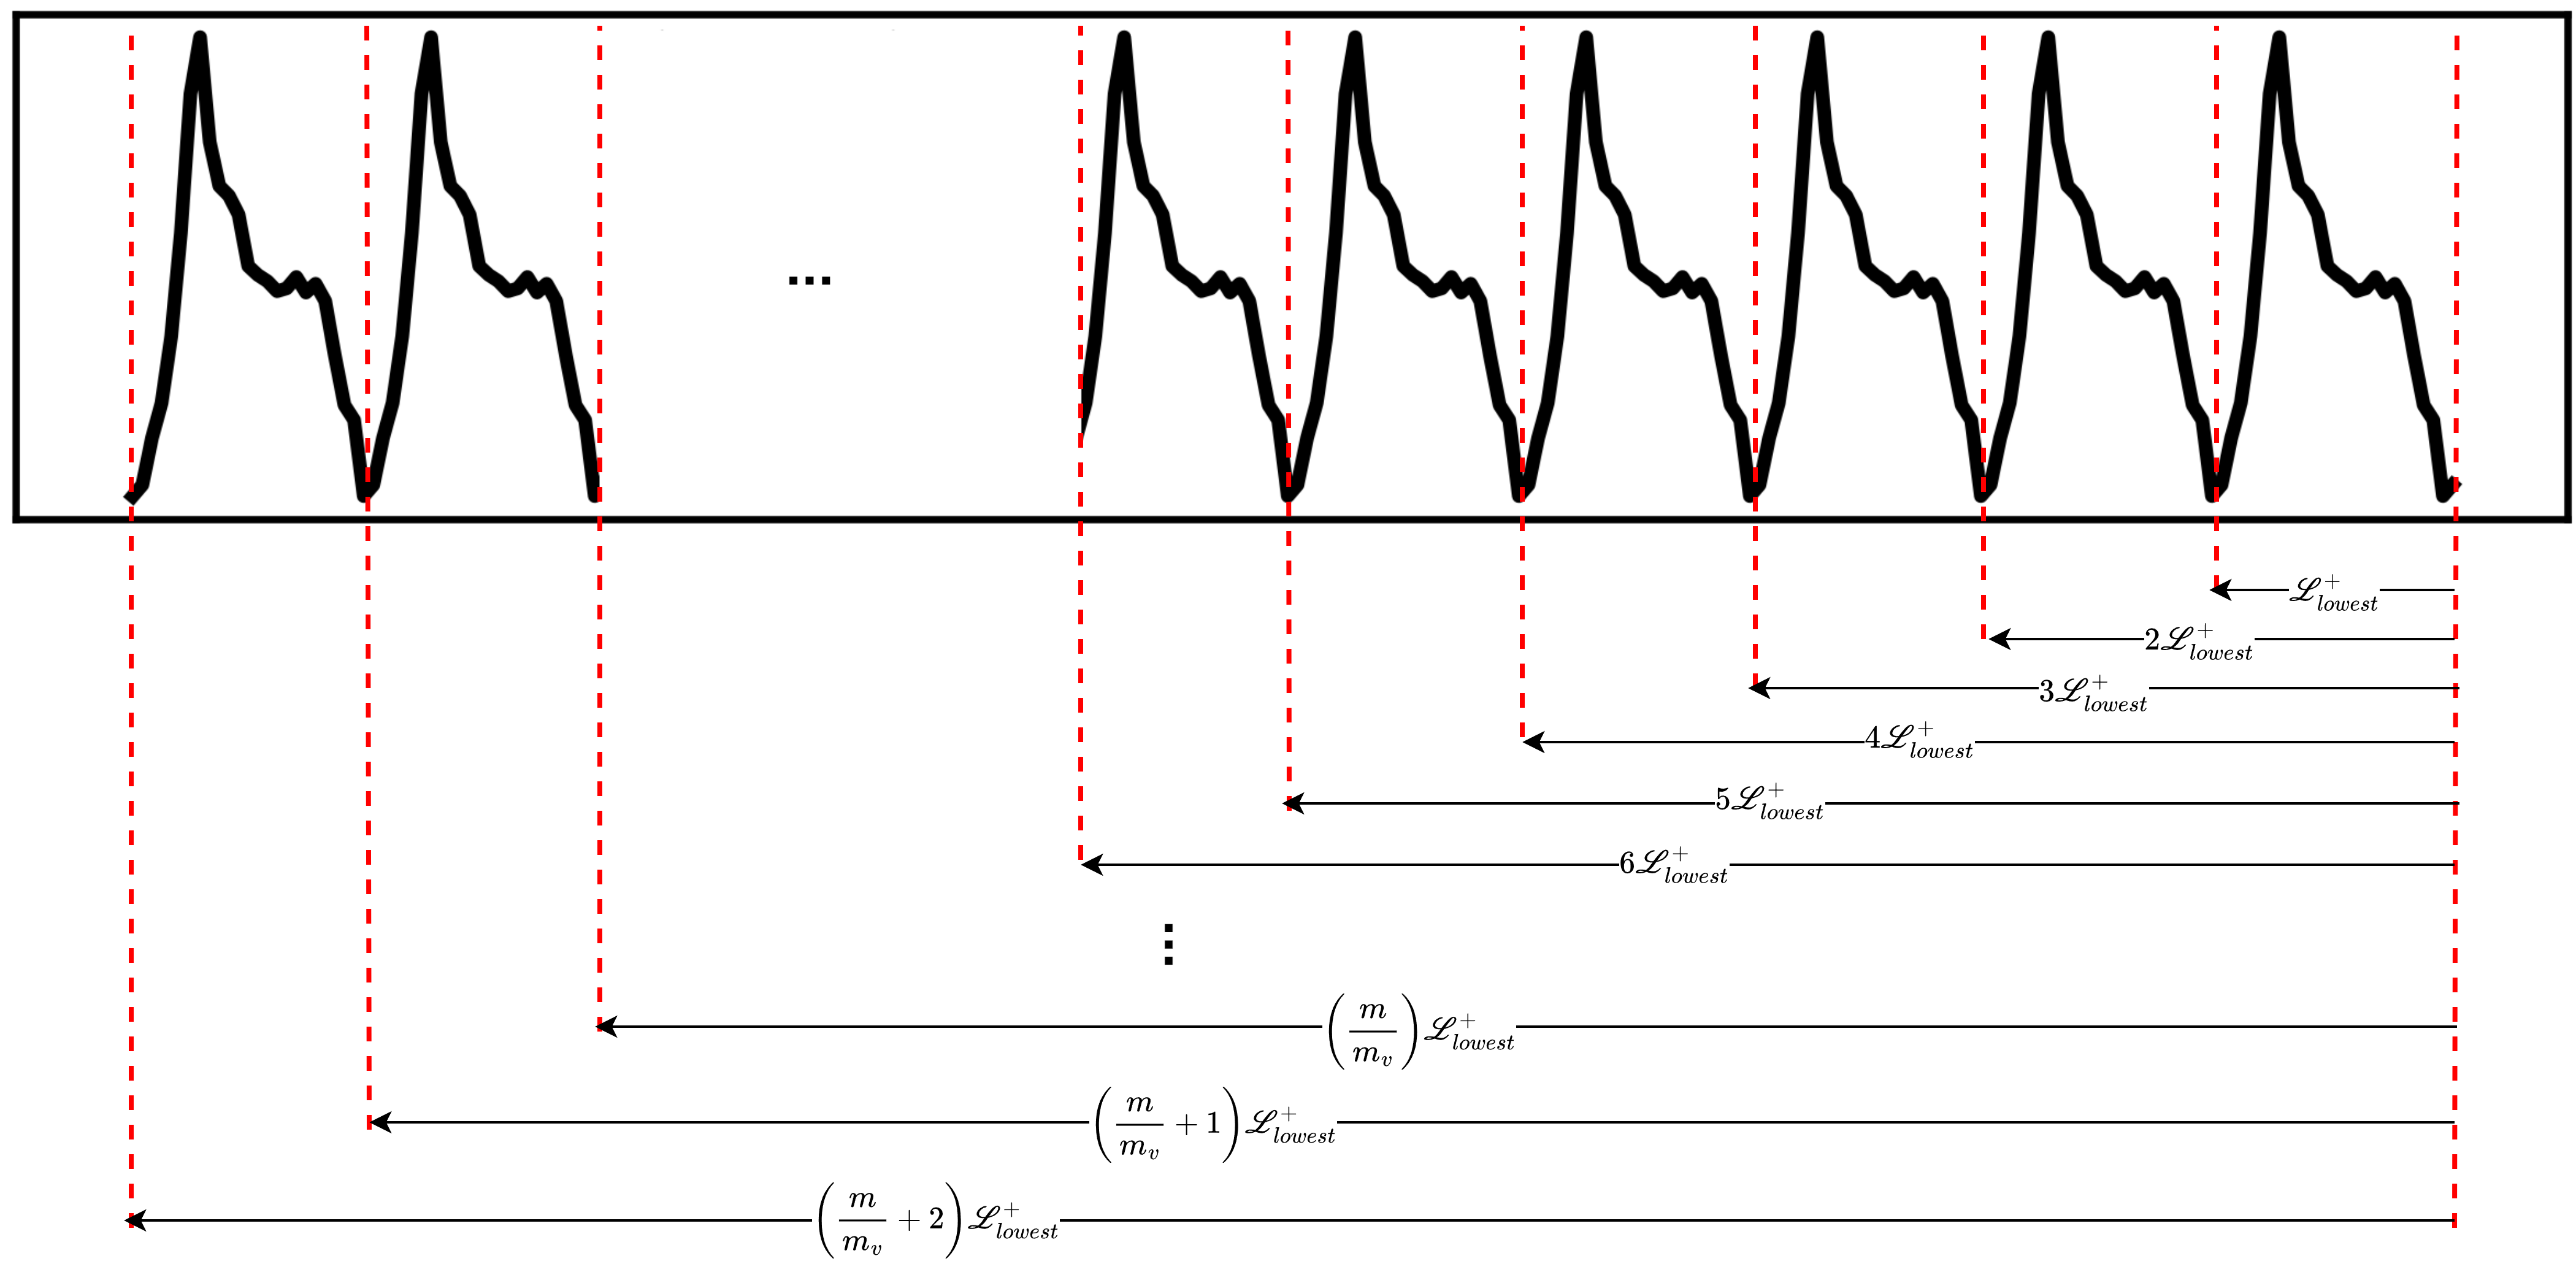
\includegraphics[scale=.6]{se_view}
  \caption{Sesisonality based view $X_v \in X$ generation.}
 \end{figure}


\item \textbf{Stacked CNN-BiLSTM : } \\
1D CNN layer for forward propagation is expressed as \Cref{1dcnn} : 
\begin{equation} \label{1dcnn}
  x_{(i, l)}^{(k, v)}=b_{(i, l)}^{(k, v)} + \sum_{j=1}^{L_{(l-1)}} conv1D \left(W_{(j, (l-1))}^{(k, v)},  S_{(j, (l-1))}^{(k, v)} \right)
\end{equation}
$L_{(l-1)}$ :  Number of neurons weight at $(l-1)$ layer.

$x_{(i, l)}^{(k, v)}$ :  $i^{th}$ input at $l$-layer of $v^{th}$ view $X_v^k$ for partion  $k$,  i.e.,  $x_{(i, l)}^{(k, v)} \in X_v^k$

$b_{(i, l)}^{(k, v)}$ :  defined as bias at $l$-layer.

$S_{(j, (l-1))}^{(k, v)}$ :  output of $j^{th}$ neurons at layer $(l-1)$.

$W_{(j, (l-1))}^{(k, v)}$ :  Kernal from the $j^{th}$ neuron at layer $(l-1)$.

$Conv1D (.)$ :  perform "in-valid" 1D convolution without zero padding.

And intermediate output $\hat{x}_{(i, l)}^{(k, v)}$ can be written as \Cref{1dd} :  
\begin{equation} \label{1dd}
  \hat{x}_{(i, l)}^{(k, v)}= f\left( x_{(i, l)}^{(k, v)} \right)
\end{equation}

In back-propagation,  the weight and bias are updated as follows : 
\begin{equation} \label{backp}
  W_{(i, (l-1))}^{(k, v)} (t+1) =W_{(i, l)}^{(k, v)}(t)- \varepsilon \frac{\partial E}{\partial W_{(i, (l-1))}^{(k, v)}}
\end{equation}

and 

\begin{equation} \label{bias}
  b_l^{(k, v)} (t+1) = b_l^{(k, v)}(t)- \varepsilon \frac{\partial E}{\partial b_l^{(k, v)}}
\end{equation}

where $\frac{\partial E}{\partial W_{(i, l-1)}^{(k, v)}} =conv1D \left(S_l^{(k, v)},  \Delta_{(l+1)}^{(k, v)} \right)$ and $\frac{\partial E}{\partial b_l^{(k, v)} }=\sum_{n}^{}\Delta_{l} (n)$. 
Then,  the find out come $\hat{x}_l^{(k, v)}$ of the 1DCNN may be written as \Cref{1dd hat}.

\begin{equation} \label{1dd hat}
  \hat{x}_l^{(k, v)}=\mathbb{F} \left(\hat{x}_{(i, l)}^{(k, v)} \right )
\end{equation}

where $\mathbb{F}(.)$ is activation function at last layer of the network. Now,  the input gate of BiLSTM can have $\hat{x}_i^{(k, v)}$ output of 1DCNN as input of BiLSTM shown in \Cref{si}.

\begin{equation}
\label{si}
  i_t^f = \sigma \left(W_{\left(\hat{x}_i^{(k, v)} \right)}^f  \bullet \hat{x}_i^{(k, v)} +W_{h_i}^f \bullet h_{(t-1)}^f +W_{c_i}^f \bullet c_{(t-1)}^f +b_i^f \right)
\end{equation}

Then ,  the final output gate can have output $\theta _{(t, 1)}^{(k, v)}$ for the fist stack

\begin{equation} \label{thi fin}
  \hat{y}_t^{(k, v)}=\theta _{(t, stack)}^{(k, v)}= \sigma \left(W_{\hat{x}_{out}^{(k, v)}} \bullet \hat{x}_{out}^{(k, v)} +  W_{h_{out}} \bullet h_t +W_{h_{out}} \bullet c_t +b_{out} \right)
\end{equation}

The stacked CNN-BiLSTM include the repetition of the same architecture that is shown from \Cref{1dcnn} to \Cref{thi fin}. Then the second stack output $\theta _{(t, 2)}^{(k, v)}$ can be obtained as \Cref{thi fin} which will corrosponding  to $v^{th}$ view of $x$ for $k$-partion. 



  \item \textbf{Multi-view Stacked CNN-BiLSTM Prediction : }\\
  The prediction of $v_{th}$ view $X_v \in X$ for $k$-partitioning is $\theta_{(t, 2)}^{(k, v)} $, so weighted ensemble of all view output for time $t$ is denoted as in \Cref{sta cb} .
  \begin{equation} \label{sta cb}
    \hat{y}_t^k= \left(\frac{1}{k} \right) \sum_{v=1}^{k} \left(\hat{y}_t^{(k, v)} \times \omega_v \right)
  \end{equation}
  where $\omega_v$ is the weight of view, i.e.,  the performance of stacked CNN-BiLSTM over validation set of $X$. over $v^{th}$ view $X_v$.



  \item \textbf{Finding best views of multi-view for learning of stacked CNN-BiLSTM : }
  Let a set of final prediction of $k$-partition of X is denoted as  $\left\{\hat{y}_t^k \right\}_{k=\mathscr{L}_{lowest}^+}^{\mathscr{L}_{lowest}^+}$ and $\mathcal{M}_k(.)$ function to measure the performance of $k$-partition (for minimization). Then,  the best views $k_{best}$ can be exhibits as \Cref{bv}
  \begin{equation} \label{bv}
    %k_{best}=arg min_{t \in T} \left\{\mathcal{M}_k \left(\hat{y}_t^k \right) \right\}_{k=\mathscr{L}_{lowest}^+}^{\mathscr{L}_{highest}^+}
    k_{best}=\underset{t \in T}{arg min} \left\{\mathcal{M}_k \left(\hat{y}_t^k \right) \right\}_{k=\mathscr{L}_{lowest}^+}^{\mathscr{L}_{highest}^+}
  \end{equation}
  where $\mathscr{L}_{lowest}^+$ and $\mathscr{L}_{highest}^+$ are minimum and maximum of $\rho_{\mathscr{L}}^+$ ACF coefficient.

\end{enumerate}


\subsubsection{Proposed Multi-view Stacked CNN-BiLSTM (MvS CNN-BiLSTM)}
% Figure
\begin{figure*}[h!]
	\centering
		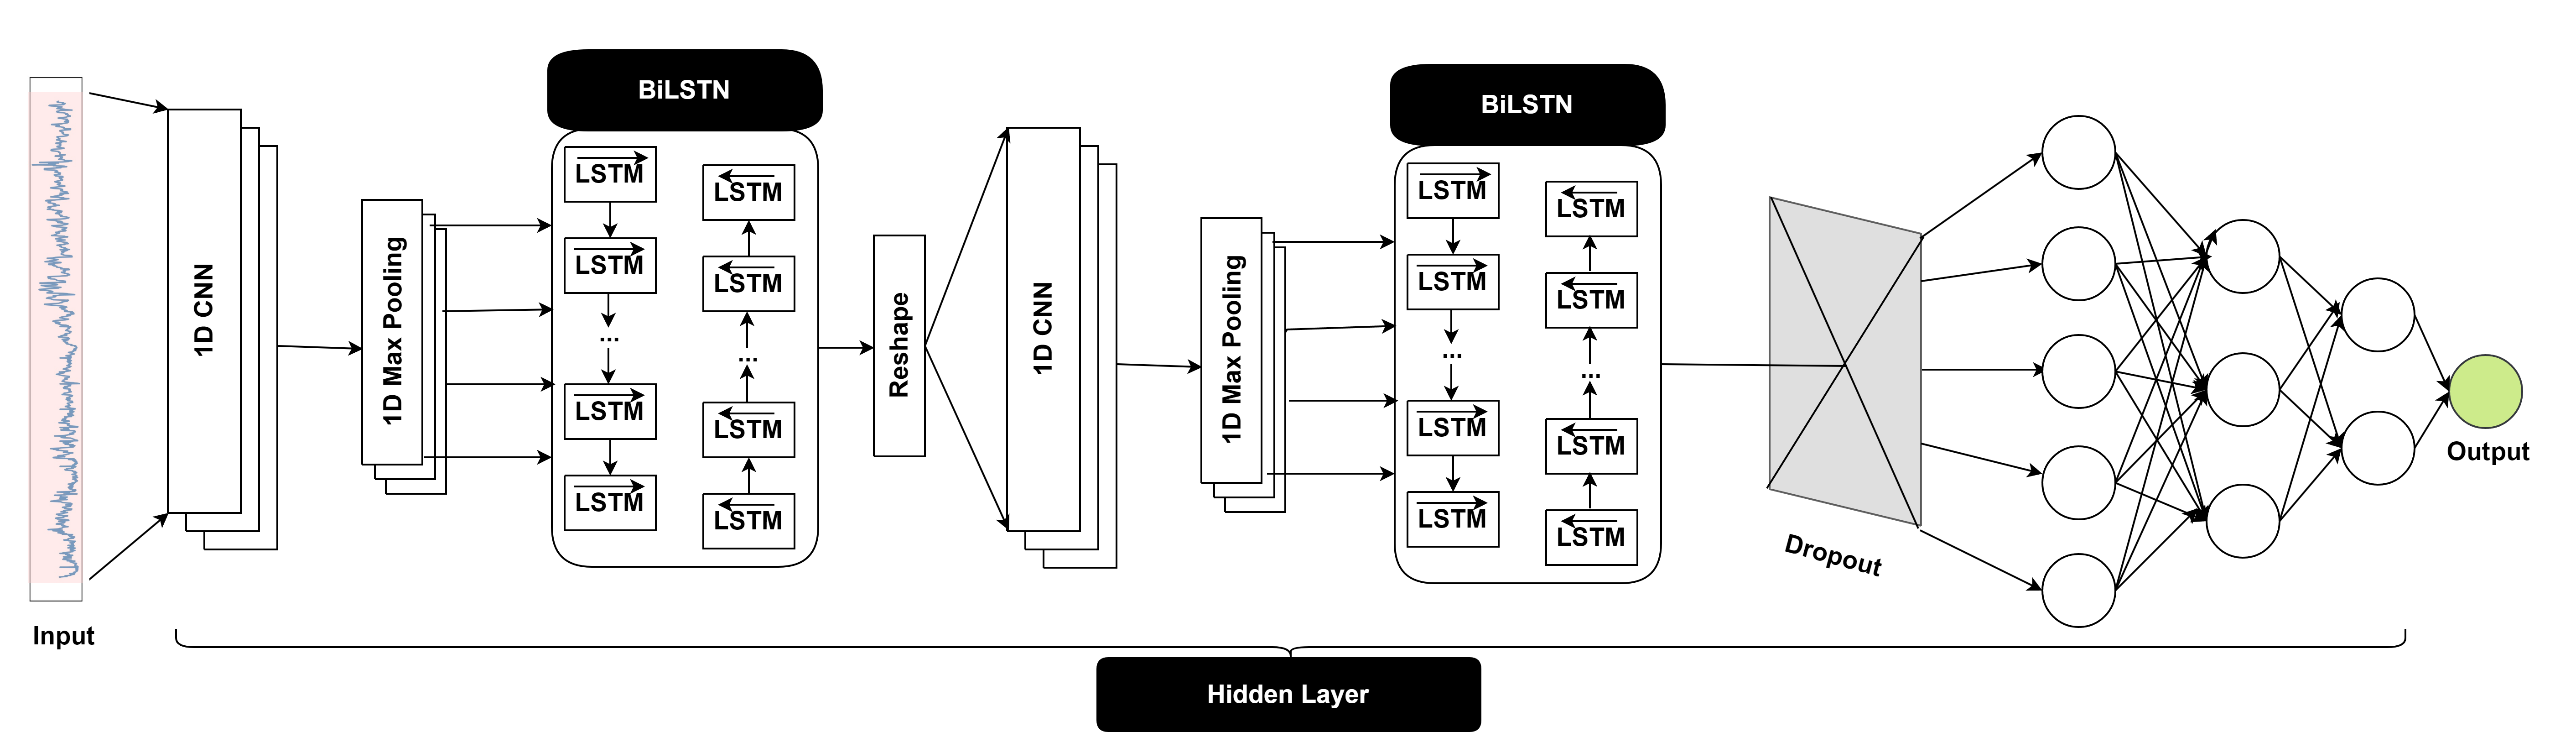
\includegraphics[scale=0.45]{Prpose}
	  \caption{Architecture of Stacked CNN-BiLSTM}\label{prosed_cnn-bilstm}
\end{figure*}

The model consists of various layers,  starting with a 1D Convolutional layer with 128 filters,  followed by a MaxPooling layer for downsampling. Next,  a Bidirectional LSTM layer with 64 units and '\textcolor{red}{ReLU}' activation is applied,  returning only the last output. A Reshape layer is introduced to reshape the output, and another 1D Convolutional layer with 32 filters is utilised,  followed by another MaxPooling layer. Another Bidirectional LSTM layer with 32 units and '\textcolor{red}{ReLU}' activation is added, returning only the last output. To prevent overfitting,  a Dropout layer with a rate of 0.2 is introduced before the final Dense layer,  which contains a single neuron for regression predictions. The model is given the name 'stacked CNN-BiLSTM'.

\subsubsection{Implamentation setup and parameters settings}
The various Python packages are utilised to implement the proposed and baseline models. These assortments incorporate Keras (v2.12.0),  TensorFlow (v2.12.0) for Keras backend,  scikit-learn (v1.2.2) for model building and performance analysis,  Pandas (v1.5.3) \& NumPy (v1.23.5) for exploratory data analysis,  and matplotlib (v3.7.1),  seaborn (v0.12.2) \& Plotly (v5.14.1) for representing the results and plotting graphs.Additionally,  It have utilized \href{https: //app.diagrams.net/}{https: //app.diagrams.net/} for creating flowcharts. Two unique systems were employed for the experiments:  a Windows-based computer with an Intel\textregistered ~Core\texttrademark ~i7-11800H \texttt{@} 2.30GHz 8 GB RAM and a Kali Linux machine with an Intel\textregistered ~Core\texttrademark ~i7-4600U \texttt{@} 2.2GHz 16 GB RAM running JupyterLab (v4.0.1).


\begin{table*}[h!]
  \caption{Parameter setting of traditional DL models and proposed MvS CNN-BiLSTM }
  \label{tab: my-table}
  \begin{tabular}{ll}
  \hline Hyperparameters & Values        \\ \hline
  Batch Size               & 66                     \\
  Optimizer                 & Adam                   \\
  Loss function            & Mean Squared Error      \\
  Epoch                    & 250 with early stopping \\
  activation function      & \textcolor{red}{ReLU}                   \\
  training size             & 0.8                   \\ \hline
  \end{tabular}
  \end{table*}


\newcommand\mycommfont[1]{\footnotesize\ttfamily\textcolor{blue}{#1}}
\SetCommentSty{mycommfont}
\SetKwInput{KwInput}{Input}                % Set the Input
\SetKwInput{KwOutput}{Output}              % set the Output

\begin{algorithm}[!ht]
  \DontPrintSemicolon
  
    \KwInput{ $X=[x_1, x_2, x_3,  \dots , x_m] $,  where $x_i \in X$, $X \in \mathbb{R}^m$ and follows the ergodic properties.\\ $K \in \mathbb{N}^+$ \tcp*{no. of partition of series $X$ and ($v=1, 2, 3, 4 \dots$)} }
    \KwOutput{$X_v^k = [x_{(1, v)}, x_{(2, v)}, x_{(3, v)},  \dots , x_{(m_v, v)}]$,  where $x_i \in X_v^k$ \& $X_v^k \subset X$,  $m_v < m$  \tcp*{$v^{th}$ $k$- no. of partition of $X$ series.} }
    
  Initialization:  $k \in \mathbb{N}^+$\\ 
  indentfying seasional for lower lag $\mathscr{L}$ using ACF coefficient $\rho_{\mathscr{L}}$ :  
  $\rho_{\mathscr{L}}=\frac{E (x_t-\mu) (x_{t+\mu} -\mu)}{\sigma_x^2}$ \tcp*{see \Cref{rovh}}
  Finding set of positive coefficient of ACF $\rho_{\mathscr{L}^+}$ :  
  $\rho_{\mathscr{L}^+}= \left\{\rho_{\mathscr{L}} > 0 \right\}_{(\mathscr{L}=1)}^{ \left| \rho_{all} \right|}$ \tcp*{see \Cref{rhl}}
  obtaining the lowest lag $\mathscr{L}_{lowest}^+$ :  
  $ \mathscr{L}_{lowest}^+ = \underset{\mathscr{L} \in \mathbb{R}}{arg min} \left\{\rho_{\mathscr{L}}^+  \right\}$ \tcp*{see \Cref{lxl}}
  Generation of $v^{th}$ view $X_v^k \in X$ for $k$-partion :  
  $T_k=\frac{(T_X)}{T_{ \mathscr{L}_{lowest}^+ }\times k}$ \tcp*{see \Cref{vvtk}}
  $X_v^k = [x_{(1, v)}, x_{(2, v)}, x_{(3, v)},  \dots , x_{(m_v, v)}]$

  Return ($X_v^k$)\\
  End
  \caption{Generation of multiple views from univariate time series $X$.}\label{alg1}
  \end{algorithm}
  


  \begin{algorithm}[!ht]
    \DontPrintSemicolon
    
      \KwInput{ $X_v^k = [x_{(1, v)}, x_{(2, v)}, x_{(3, v)},  \dots , x_{(m_v, v)}]$ \tcp*{fron \Cref{alg1} }}
      \KwOutput{$\theta _{(t, 2)}^{(k, v)}$ \tcp*{output  at second stack of CNN-BiLSTM}}
      
    Initialization:  stack = 1\\ 
    \If{stack $\le$ 2}{
      1DCNN layer for forward propagation:   
       $x_{(i, l)}^{(k, v)}=b_{(i, l)}^{(k, v)} + \sum_{j=1}^{L_{(l-1)}} conv1D \left(W_{(j, (l-1))}^{(k, v)},  S_{(j, (l-1))}^{(k, v)} \right)$ \tcp*{see \Cref{1dcnn}}
      outcome of 1DCNN from last layer using activation function $\mathscr{F}(.)$ :  
      $\hat{x}_l^{(k, v)}=\mathbb{F} \left(\hat{x}_{(i, l)}^{(k, v)} \right )$ \tcp*{see \Cref{1dd hat}}
      The output of the previous step-2 is the input of the BiLSTM input Gate (forward) :  
      $i_t^f = \sigma \left(W_{\left(\hat{x}_i^{(k, v)} \right)}^f  \bullet \hat{x}_i^{(k, v)} +W_{h_i}^f \bullet h_{(t-1)}^f +W_{c_i}^f \bullet c_{(t-1)}^f +b_i^f \right)$ \tcp*{see \Cref{si}}
      Then output of BiLSTM $\theta_{(t,  stack)}^{(k, v)}$ can be recived as :  
      $\theta _{(t, stack)}^{(k, v)}= \sigma \left(W_{\hat{x}_{out}^{(k, v)}} \bullet \hat{x}_{out}^{(k, v)} +  W_{h_{out}} \bullet h_t +W_{h_{out}} \bullet c_t +b_{out} \right)$ 
      Repeat step-2 to 6 for stack=2; then the final output can be written as : 
      $\hat{y}_t^{(k, v)}=\theta _{(t, stack)}^{(k, v)}= \sigma \left(W_{\hat{x}_{out}^{(k, v)}} \bullet \hat{x}_{out}^{(k, v)} +  W_{h_{out}} \bullet h_t +W_{h_{out}} \bullet c_t +b_{out} \right)$  \tcp*{see \Cref{thi fin}}

    }
    Return ($\hat{y}_t^{(k, v)}$)\\
    End
    \caption{Stacked CNN-BiLSTM Model.}\label{alg2}
    \end{algorithm}



  \begin{algorithm}[!ht]
    \DontPrintSemicolon
      
      \KwInput{$X=[x_1, x_2, x_3,  \dots , x_m] $,  $x_i \in X$, $X \in \mathbb{R}^m$ \tcp*{Time series data (univariate).}\\ $K \in \mathbb{N}^+$ \tcp*{no. of partition of series $X$}.}
      \KwOutput{$\hat{y}_t^k$ \tcp*{Find weight aggregation of all output of model induced from views $X_v$}}
        
    Initialization:  $K \in \mathbb{N}^+$,  $\hat{y}_t^{(k, v)}= \left\{\phi \right\}$\\ 
    Checking ergodicity of univariate time series $X$ after preprocessing.\\
    Find the strength of seasonality of $X$ as $F_s$ : 
      $F_S=max \left(0, 1- \frac{Var (X^R)}{Var(X^S + X^R)} \right)$ \tcp*{see \Cref{fs}}
    \If{($F_s$ > 0)}{
      \For{$v=1$ to $k$ : }{
        Generating the $v^{th}$ view for $k$- partition from \Cref{alg1} i.e. $X_v^k$  \\
        Deployment of CNN-BiLSTM model \Cref{alg2} for the input series $X_v^k$,  then output recieved i.e. $\hat{y}_t^{(k, v)'}$ \\
        update the set of prediction of model induced with $v^{th}$ view $X_v^k$ as: 
        $\hat{y}_t^{(k, v)} \gets \left\{\hat{y}_t^{(k, v)}  \right\}  \cup \left\{\hat{y}_t^{(k, v)'}  \right\}$
      }
      Weighted aggregation of view-wise model prediction to get the find output $\hat{y}_t^k$ as: 
      $\hat{y}_t^k= \left(\frac{1}{k} \right) \sum_{v=1}^{k} \left(\hat{y}_t^{(k, v)} \times \omega_v \right)$ \tcp*{see \Cref{bv}}
    }
    Return ($\hat{y}_t^k$)\\
    End
    \caption{Stacked CNN-BiLSTM Model.}\label{alg3}
  \end{algorithm}



\section{Results and Discussion}


% Figure
\begin{figure*}[h!]
	\centering
		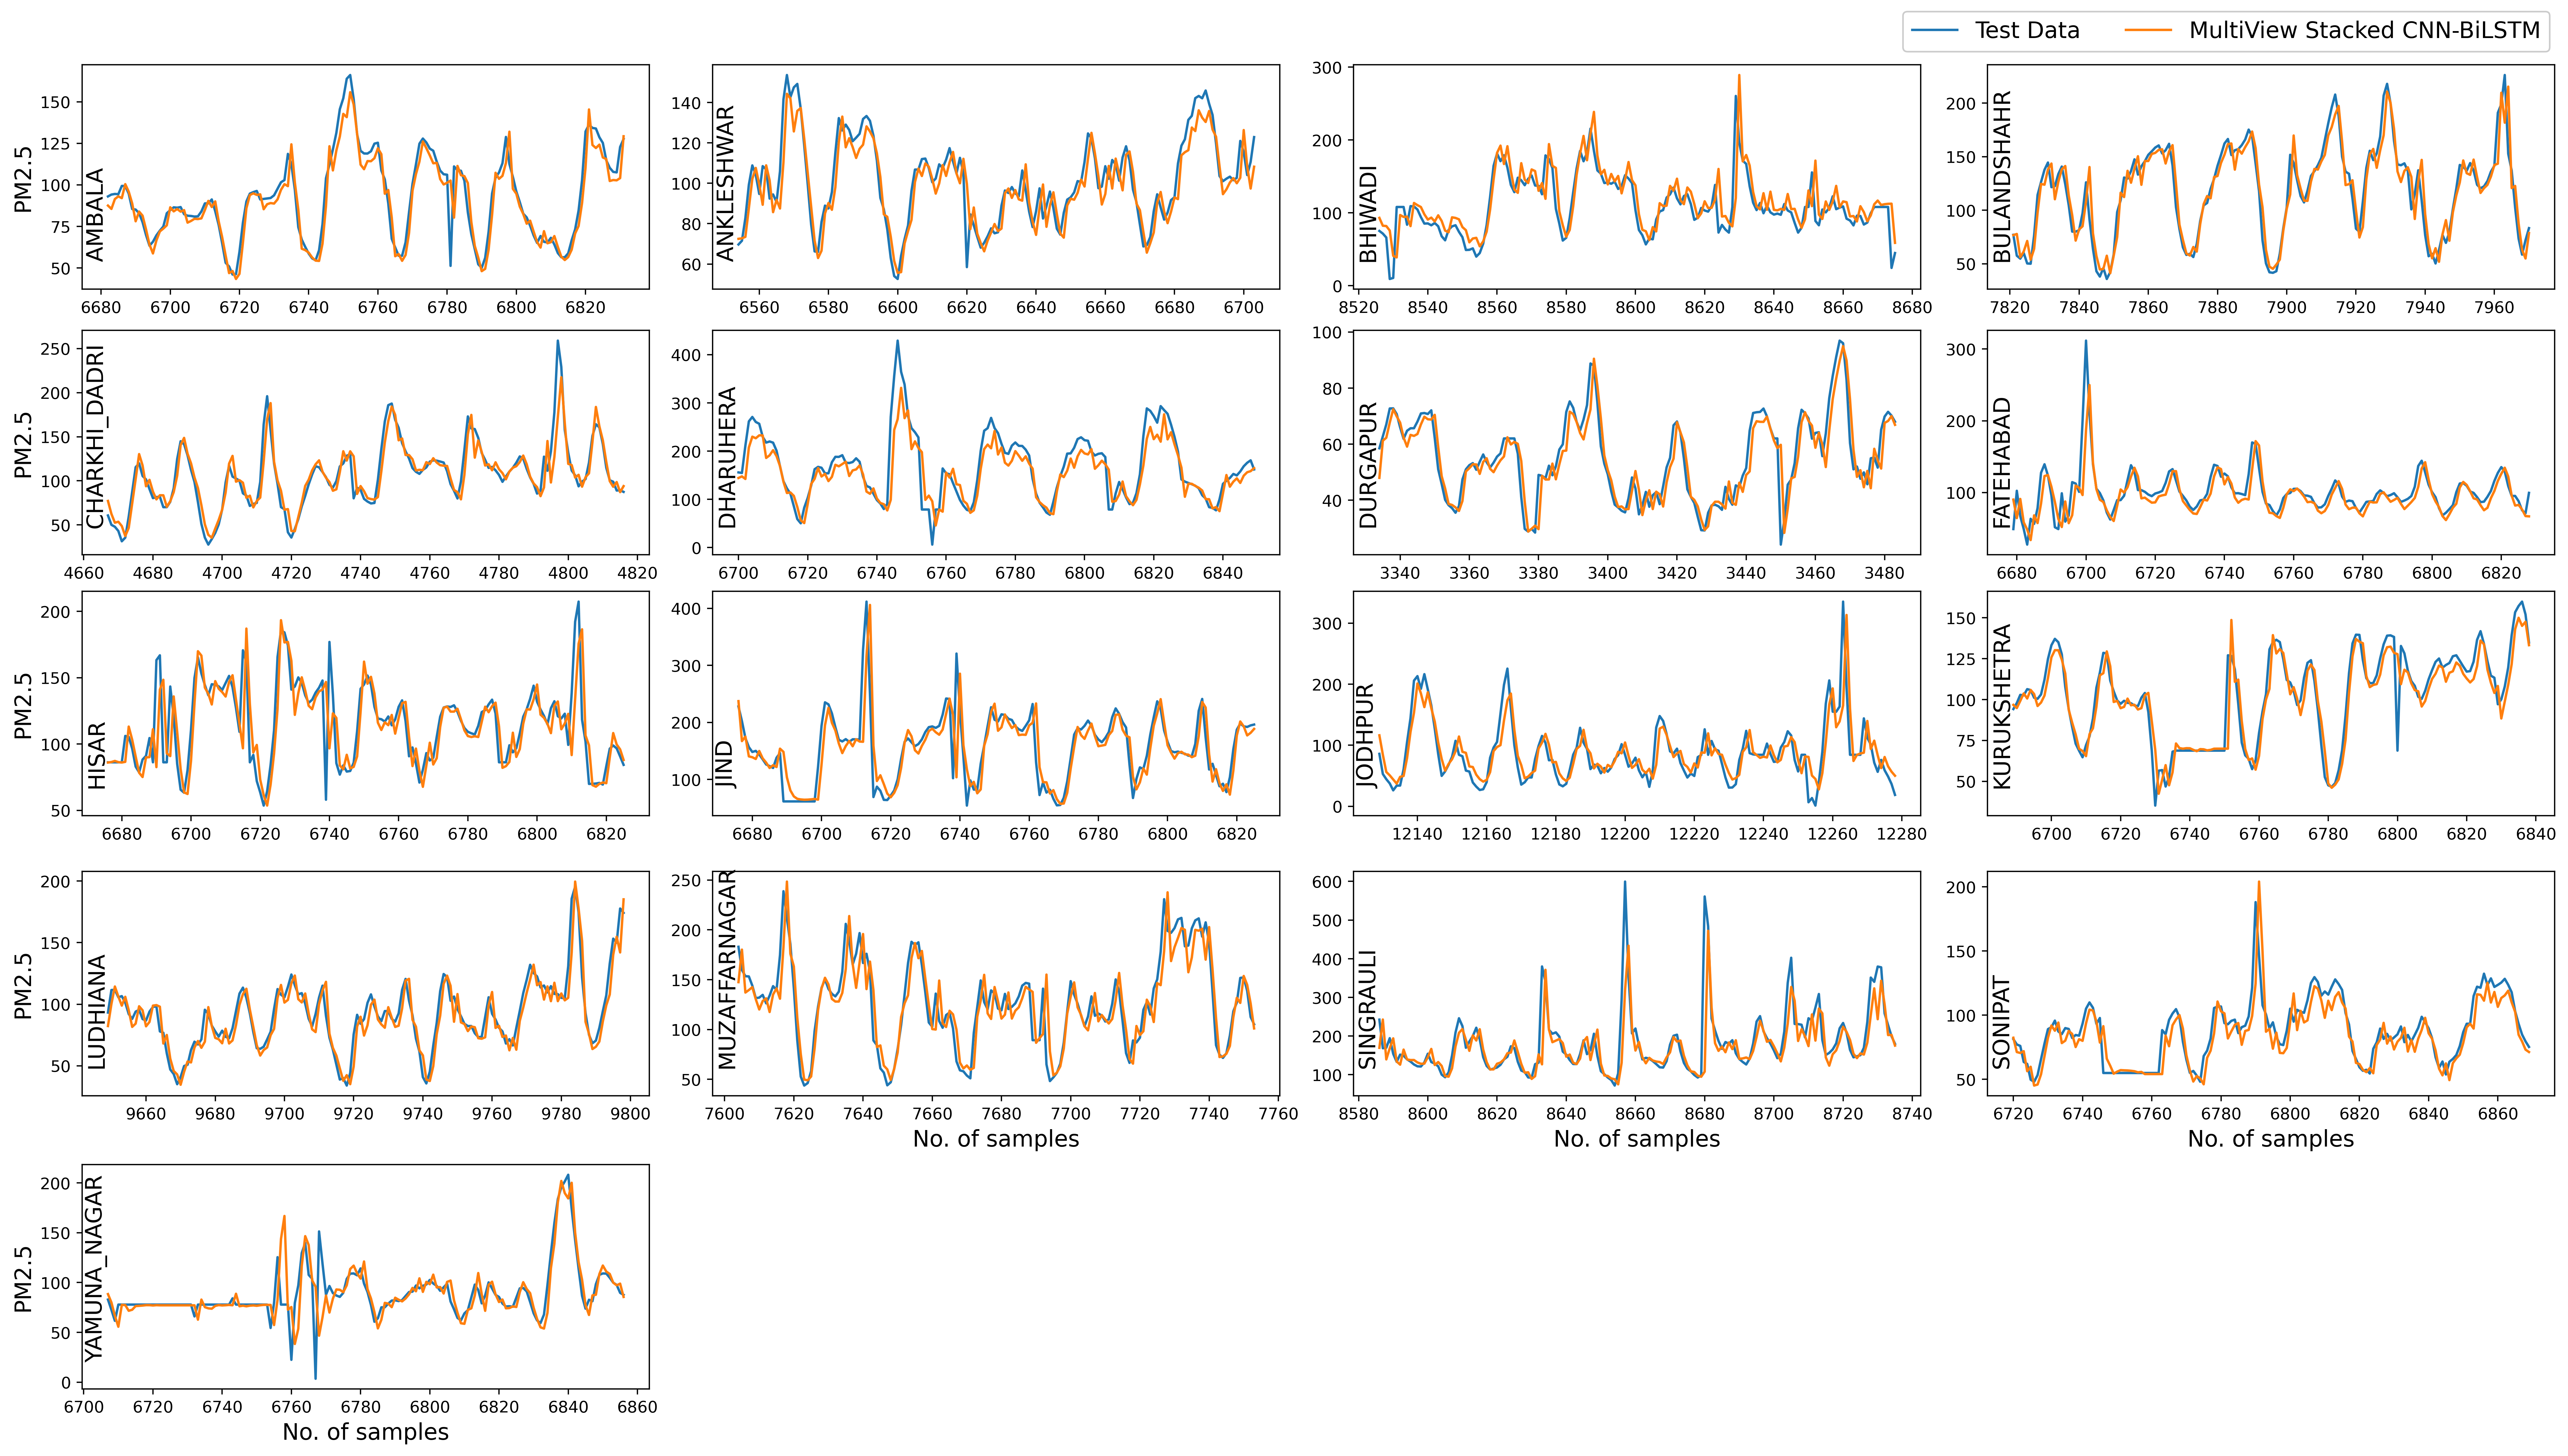
\includegraphics[scale=0.29]{act vs pri}
	  \caption{$PM_{2.5}$ predictions of proposed models MvS CNN-BiLSTM}\label{ACt_vs_Pred}
\end{figure*}
\Cref{ACt_vs_Pred} depicts a series of subplots that illustrate different datasets,  each showcasing the comparison between the predicted and actual $PM_{2.5}$ values on the test dataset. The x-axis indicates the quantity of data points,  while the $PM_{2.5}$ values are represented by the y-axis. Every subplot is associated with a specific dataset name,  signifying the MvS CNN-BiLSTM model's evaluation performance on various datasets,  which may reflect different time periods or locations where $PM_{2.5}$ concentrations were monitored and documented. In each subplot,  the test dataset's samples are represented by data points. For each data point,  there are two values plotted:  the actual $PM_{2.5}$ value (ground truth) and the corresponding predicted $PM_{2.5}$ value generated by the MvS CNN-BiLSTM model. The plot allows us to visually compare how well the model's predictions match the actual values for each dataset. In \Cref{ACt_vs_Pred}, the "prediction mimicking test" refers to comparing the model's predicted values with the actual values in the test dataset to assess the accuracy and effectiveness of the predictive model.





% Please add the following required packages to your document preamble: 
% \usepackage{graphicx}
\begin{table}[]
  \caption{RMSE Performance of traditional DL models and proposed models $($ MvS CNN-BiLSTM$)$.}
  \label{tab: RMSE}
  \resizebox{\textwidth}{!}{%
  \begin{tabular}{llllllcc}
 \hline DataSet        & BiLSTM  & CNN & GRU      & LSTM & RNN       & MvS CNN-BiLSTM        & Best-view \\ \hline
AMBALA         & 33.382          & 36.239    & \textbf{33.012} & 33.136     & 33.455                & 33.272          & 4      \\
ANKLESHWAR     & 22.916          & 23.724    & 22.975          & 23.359     & 22.807                & \textbf{22.081} & 6      \\
BHIWADI        & 28.043          & 25.168    & 25.521          & 26.512     & 25.974                & \textbf{24.959} & 10     \\
BULANDSHAHR    & 16.155          & 16.894    & \textbf{14.807} & 16.001     & 14.923                & 16.265          & 7      \\
 DCHARKHI\_DADRI & \textbf{30.071} & 32.709    & 32.299          & 32.629     & 33.836              & 31.064          & 3      \\
 DHARUHERA      & 25.751          & 26.948    & 26.057          & 26.108     & 25.489           &\textbf{24.983}          & 3      \\
 DURGAPUR       & 10.426          & 9.719     & 11.375          & 11.994     & 10.664                    & \textbf{8.906}  & 6      \\
 FATEHABAD      & 31.501          & 31.251    & 32.169          & 31.045     & 30.946                    & \textbf{30.86}  & 10     \\
 HISAR          & 21.677          & 22.286    & 20.875          & 21.371     & 21.617                 & \textbf{20.155} & 6      \\
 JIND           & 26.619          & 26.29     & 25.043          & 24.813     & \textbf{24.364}           & 24.408          & 10     \\
 JODHPUR        & 27.749          & 27.617    & 27.787          & 27.519     & 27.951              & \textbf{27.482} & 7      \\
 KURUKSHETRA    & 16.475          & 16.352    & 15.239          & 17.359     & \textbf{15.414}           & 15.921          & 5      \\
 LUDHIANA       & 14.573          & 17.013    & \textbf{13.817} & 17.668     & 14.936                    & 14.315          & 9      \\
 MUZAFFARNAGAR  & 20.885          & 23.182    & 21.206          & 20.412     & 23.638                   & \textbf{19.859} & 10     \\
 SINGRAULI      & 33.995          & 36.569    & \textbf{32.993} & 33.142     & 35.572                    & 33.834          & 2      \\
 SONIPAT        & 13.644          & 13.951    & 14.025          & 13.773     & 13.755                    & \textbf{12.75}  & 5      \\
 YAMUNA\_NAGAR  & 31.985          & 36.433    & 32.413          & 32.699     & 35.591                    & \textbf{31.676} & 8     \\ \hline
  \end{tabular}%
  }
  \end{table}
  \Cref{tab: RMSE} exhibits the RMSE performance of different conventional DL models and the proposed MvS CNN-BiLSTM model on 17 datasets. The graph emphasises the random-performing model (i.e.,  the model with unpredictable RMSE) for each dataset using strikethrough text. The leftmost column lists the names of the evaluated datasets,  while the next columns represent the RMSE values of different traditional DL models on each dataset. The proposed MvS CNN-BiLSTM model's RMSE values are displayed in the "MvS CNN-BiLSTM" column. The "Best-view" column identifies the DL model that achieved the lowest RMSE on each dataset,  highlighted using bold text.

  The table thoroughly compares various DL models' RMSE performance across multiple datasets,  with the MvS CNN-BiLSTM model demonstrating better RMSE values in its respective column and the bolded values indicating the best-performing model for each dataset.
  
  \Cref{tab: RMSE} provides valuable insights into the predictive capabilities of traditional DL models and the proposed MvS CNN-BiLSTM model. The MvS CNN-BiLSTM model for better performance over several traditional deep learning models on diverse datasets,  as evidenced by the lower RMSE values. The highlighted values help identify the best model for each dataset,  highlighting the effectiveness of the proposed MvS CNN-BiLSTM approach over traditional DL models.


  \begin{table}[]
    \caption{\textcolor{red}{Percentage improvement of MvS CNN-BiLSTM respectively BiLSTM,  CNN,  GRU,  LSTM and RNN on RMSE.}}
    \label{RMSE imp}
    \begin{tabular}{lccccc}
    \hline    Dataset        &   BiLSTM &   CNN &   GRU &   LSTM &   RNN \\ \hline
    AMBALA & 0.33\% & 8.19\% & -0.79 \% & -0.41\% & 0.55\% \\
    ANKLESHWAR & 3.64\% & 6.93\% & 3.89\% & 5.47\% & 3.18\% \\
    BHIWADI & 11.00\% & 0.83\% & 2.20\% & 5.86\% & 3.91\% \\
    BULANDSHAHR & -0.68\% & 3.72\% & -9.85\% & -1.65\% & -8.99\% \\
    CHARKHI\_DADRI &-3.3\% & 5.03\% & 3.82\% & 4.80\% & 8.19\% \\
    DHARUHERA & 2.98\% & 7.29\% & 4.12\% & 4.31\% & 1.99\% \\
    DURGAPUR & 14.58\% & 8.37\% & 21.71\% & 25.75\% & 16.49\% \\
    FATEHABAD & 2.03\% & 1.25\% & 4.07\% & 0.60\% & 0.28\% \\
    HISAR & 7.02\% & 9.56\% & 3.45\% & 5.69\% & 6.76\% \\
    JIND & 8.31\% & 7.16\% & 2.54\% & 1.63\% & -0.18\% \\
    JODHPUR & 0.96\% & 0.49\% & 1.10\% & 0.13\% & 1.68\% \\
    KURUKSHETRA & 3.36\% & 2.64\% & -4.48\% & 8.28\% & -3.29\% \\
    LUDHIANA & 1.77\% & 15.86\% & -3.6\% & 18.98\% & 4.16\% \\
    MUZAFFARNAGAR & 4.91\% & 14.33\% & 6.35\% & 2.71\% & 15.99\% \\
    SINGRAULI & 0.47\% & 7.48\% & -2.55\% & -2.09\% & 4.89\% \\
    SONIPAT & 6.55\% & 8.61\% & 9.09\% & 7.43\% & 7.31\% \\
    YAMUNA\_NAGAR & 0.97\% & 13.06\% & 2.27\% & 3.13\% & 11.00\% \\ \hline
    \textbf{Positive Avg}  & \textbf{4.05\%} & \textbf{7.11\%}& \textbf{3.80\%} & \textbf{5.57\%} & \textbf{5.08\%} \\ \hline
    \end{tabular}
    \end{table}
  \Cref{RMSE imp} illustrates the extent $\%$ of improvement from conventional deep learning (DL) models to the proposed MvS CNN-BiLSTM model across 17 datasets. The chart showcases the growth rate of every deep learning model,  namely BiLSTM,  CNN,  GRU,  LSTM,  and RNN, concerning the MvS CNN-BiLSTM model. Negative values indicate that the corresponding DL model outperformed the MvS CNN-BiLSTM model for a particular dataset. The table consists of a pair of columns that are connected. The right column depicts the percentage of regression for the multivariate effective CNN-BLSTM model compared to traditional DL models for each dataset evaluated in the study in the left column. Each dataset's corresponding percentage of improvement for each DL model is presented in their respective columns. A positive percentage value denotes that the MvS CNN-BiLSTM model performed better than the specific DL model by the percentage indicated.



\begin{table}[!htp]
  \caption{Average Rankings of the algorithms (Friedman) in a contest of RMSE.}
  \centering
  \begin{tabular}{lccc}
  \hline
  Algorithm&Ranking&$p$&Holm\\\hline
  BiLSTM&3.7059&0.002485&0.016667\\
  CNN&4.8235&0.000002&0.01\\
  GRU&3.1765&0.027801&0.05\\
  LSTM&3.8235&0.001335&0.0125\\
  RNN&3.7059&0.002485&0.025\\
  \textbf{MvS CNN-BiLSTM}&\textbf{1.7647}&$-$ &$-$ \\\hline
\end{tabular}
\label{rank_rmse}
  \end{table}
  \Cref{rank_rmse} exhibits the average rankings of various algorithms about the RMSE metric,  thereby providing insights into their relative performance. The table comprises four columns: algorithm,  Ranking,  $p$-value,  and Holm. The names of several algorithms,  including BiLSTM,  CNN,  GRU,  LSTM,  RNN,  and the recently suggested MvS CNN-BiLSTM,  are being logged in the algorithm column while the assessment process is underway. The standing column exhibits the mean ranks of every algorithm relying on their performance in terms of RMSE,  where a lesser rank indicates superior performance, with 1 being the best rank and higher numbers indicating weaker performance. Each algorithm's comparison is assigned a significance level in the $p$-value column,  with a small $p$-value indicating a statistically significant difference in performance between the compared algorithms. The Holm column controls the family-wise error rate by indicating adjusted significance thresholds utilised in multiple statistical tests. The proposed MvS CNN-BiLSTM algorithm accomplished an average ranking of 1.7647, the finest among all compared models concerning RMSE. The MvS CNN-BiLSTM algorithm was not used in comparing traditional shallow learning models (BiLSTM,  CNN,  GRU,  LSTM,  and RNN). Furthermore,  the minute $p$-values for every algorithmic comparison imply a statistically significant variance in performance amongst all the algorithms,  signifying that the performance of each algorithm is discernible from others based on the RMSE metric. The Holm column likely indicates the adjusted significance thresholds (critical values) used in the Holm method for multiple comparisons, a statistical procedure used to control the family-wise error rate when performing multiple hypothesis tests. The MvS CNN-BiLSTM algorithm is the superior choice based on the table's data,  performing better than other algorithms in RMSE.








% Please add the following required packages to your document preamble: 
% \usepackage{graphicx}
\begin{table}[]
  \caption{MAPE Performance of traditional DL models and proposed models $($MvS CNN-BiLSTM$)$.}
  \label{tab: MAPE}
  \resizebox{\textwidth}{!}{%
  \begin{tabular}{llllllcc}
 \hline DataSet        & BiLSTM  & CNN & GRU      & LSTM & RNN      & MvS CNN-BiLSTM        & Best-view \\ \hline
  AMBALA         & 54.468       & 49.153    & 76.839    & 58.619     & 53.375    & \textbf{18.73}  & 3      \\
  ANKLESHWAR     & 18.86        & 19.968    & 19.015    & 19.576     & 20.72     & \textbf{16.265} & 10     \\
  BHIWADI        & 134.448      & 118.741   & 123.123   & 127.481    & 124.503   & \textbf{20.98}  & 2      \\
  BULANDSHAHR    & 44.602       & 47.066    & 26.254    & 43.721     & 27.813    & \textbf{22.469} & 3      \\
  CHARKHI\_DADRI & 50.328       & 101.385   & 102.063   & 112.912    & 115.673   & \textbf{26.728} & 10     \\
  DHARUHERA      & 35.638       & 39.358    & 39.557    & 35.942     & 40.34     & \textbf{17.365} & 3      \\
  DURGAPUR       & 45.511       & 37.529    & 56.324    & 57.457     & 48.626    & \textbf{19.321} & 6      \\
  FATEHABAD      & 19.737       & 19.929    & 19.475    & 18.663     & 17.724    & \textbf{12.178} & 5      \\
  HISAR          & 17.971       & 18.422    & 17.988    & 17.983     & 21.475    & \textbf{15.082} & 6      \\
  JIND           & 25.945       & 30.822    & 27.344    & 24.596     & 33.464    & \textbf{16.618} & 3      \\
  JODHPUR        & 40.188       & 40.36     & 41.584    & 41.578     & 43.36     & \textbf{28.278} & 7      \\
  KURUKSHETRA    & 13.713       & 13.392    & 12.405    & 13.986     & 13.312    & \textbf{11.248} & 2      \\
  LUDHIANA       & 37.61        & 47.14     & 34.504    & 51.036     & 41.197    & \textbf{15.706} & 9      \\
  MUZAFFARNAGAR  & 24.162       & 27.253    & 23.37     & 26.08      & 27.061    & \textbf{16.571} & 5      \\
  SINGRAULI      & 48.642       & 67.143    & 39.738    & 34.372     & 68.525    & \textbf{28.545} & 7      \\
  SONIPAT        & 43.301       & 48.32     & 49.409    & 43.187     & 45.67     & \textbf{13.541} & 7      \\
  YAMUNA\_NAGAR  & 65.601       & 63.698    & 64.637    & 63.404     & 70.02     & \textbf{28.29}  & 10    \\ \hline
  \end{tabular}%
  }
  \end{table}
\Cref{tab: MAPE} showcases MAPE results of the MvS CNN-BiLSTM model and traditional DL models across 17 datasets. The DL models analysed in the table include BiLSTM,  CNN,  GRU,  LSTM,  and RNN. The MAPE values for each DL model are compared with those of the MvS CNN-BiLSTM model. The minimum MAPE values obtained by each model for each dataset and the corresponding best view are presented in \textbf{bold}. To expound the \Cref{tab: MAPE},  the initial column enumerates the names of the datasets assessed in the investigation. The succeeding columns indicate the MAPE values for the different traditional DL models compared to each dataset's proposed MvS CNN-BiLSTM model. The table's interpretation involves the presentation of the corresponding MAPE value for each DL model to their respective columns. The "Best-view" column,  on the other hand,  specifies the best dataset for which the MvS CNN-BiLSTM model obtained the minimum MAPE value. In conclusion,  \Cref{tab: MAPE} compares the MAPE performance of the MvS CNN-BiLSTM model and traditional DL models across multiple datasets. The values in \textbf{bold} highlight the MvS CNN-BiLSTM model's superior performance over traditional DL models for different datasets. The table demonstrates the MvS CNN-BiLSTM model's ability to reduce MAPE for air quality prediction in various locations and datasets.






  \begin{table}[]
    \caption{ \textcolor{red}{Improvement of MvS CNN-BiLSTM respectively BiLSTM,  GRU,  LSTM and RNN on MAPE.}}
    \label{MAPE imp}
    \begin{tabular}{lccccc}
    \hline   Dataset       &   BiLSTM &CNN & GRU &   LSTM &   RNN  \\ \hline
    AMBALA & 35.74\% & 30.42\% & 58.11\% & 39.89\% & 34.64\% \\
    ANKLESHWAR & 2.59\% & 3.70\% & 2.75\% & 3.31\% & 4.45\% \\
    BHIWADI & 113.47\% & 97.76\% & 102.14\% & 106.50\% & 103.52\% \\
    BULANDSHAHR & 22.13\% & 24.60\% & 3.78\% & 21.25\% & 5.34\% \\
    CHARKHI\_DADRI & 23.60\% & 74.66\% & 75.34\% & 86.18\% & 88.94\% \\
    DHARUHERA & 18.27\% & 21.99\% & 22.19\% & 18.58\% & 22.98\% \\
    DURGAPUR & 26.19\% & 18.21\% & 37.00\% & 38.14\% & 29.30\% \\
    FATEHABAD & 7.56\% & 7.75\% & 7.30\% & 6.48\% & 5.55\% \\
    HISAR & 2.89\% & 3.34\% & 2.91\% & 2.90\% & 6.39\% \\
    JIND & 9.33\% & 14.20\% & 10.73\% & 7.98\% & 16.85\% \\
    JODHPUR & 11.91\% & 12.08\% & 13.31\% & 13.30\% & 15.08\% \\
    KURUKSHETRA & 2.46\% & 2.14\% & 1.16\% & 2.74\% & 2.06\% \\
    LUDHIANA & 21.90\% & 31.43\% & 18.80\% & 35.33\% & 25.49\% \\
    MUZAFFARNAGAR & 7.59\% & 10.68\% & 6.80\% & 9.51\% & 10.49\% \\
    SINGRAULI & 20.10\% & 38.60\% & 11.19\% & 5.83\% & 39.98\% \\
    SONIPAT & 29.76\% & 34.78\% & 35.87\% & 29.65\% & 32.13\% \\
    YAMUNA\_NAGAR & 37.31\% & 35.41\% & 36.35\% & 35.11\% & 41.73\% \\ \hline
    \textbf{Positive Avg} & \textbf{23.11\% }& \textbf{27.16\% }& \textbf{26.22\%} & \textbf{27.22\%} & \textbf{28.52\%} \\ \hline
    \end{tabular}
    \end{table}
    \Cref{MAPE imp} displays the percentage improvement in MAPE attained by the proposed MvS CNN-BiLSTM model compared to various traditional DL models (BiLSTM,  GRU,  LSTM,  RNN) for all 17 datasets. The first column of the table lists the names of the datasets evaluated in the study. The succeeding columns represent the percentage improvement in MAPE achieved by the MvS CNN-BiLSTM model over each traditional DL model on each dataset. The percentage values in the table indicate the reduction in MAPE attained by the MvS CNN-BiLSTM model relative to each traditional DL model,  with negative values implying cases where the traditional DL model outperformed the MvS CNN-BiLSTM model.


    \begin{table}[!htp]
      \caption{Average rankings of the algorithms (Friedman) in the context of MAPE.}
      \centering
      \begin{tabular}{lccc}\hline
      Algorithm&Ranking&$p$&Holm\\\hline
      BiLSTM&3.4706&0.000118&0.05\\
      CNN&4.1765&0.000001&0.0125\\
      GRU&3.7647&0.000016&0.025\\
      LSTM&3.8824&0.000007&0.016667\\
      RNN&4.7059&0&0.01\\
      \textbf{MvS CNN-BiLSTM}&\textbf{1}&$-$ &$-$\\\hline
    \end{tabular}
      
      \label{rank_mape}
      \end{table}
      \Cref{rank_mape} showcases the average rankings of multiple algorithms in the context of the MAPE metric,  providing insight into the relative performance of these algorithms. The primary row comprises the appellation of the systems being measured,  particularly BiLSTM,  CNN,  GRU,  LSTM,  RNN,  and the purpose of MvS CNN-BiLSTM. The subsequent column displays the average rankings of each algorithm according to their MAPE performance,  with a lower ranking indicating superior performance and a greater number indicating inferior performance. The third column denotes the p-values, the significance level for comparing each algorithm. A statistically significant difference in performance between the compared algorithms is present if the $p$-value is low. The fourth column,  "Holm, " will likely denote the critical values or adjusted significance thresholds used for multiple comparisons. The Holm method manages the family-wise error rate when conducting multiple statistical tests.
      
      The MvS CNN-BiLSTM algorithm is better regarding MAPE,  surpassing all other models,  including BiLSTM,  CNN,  GRU,  LSTM,  and RNN,  with an average rank of 1. It is thus improbable to assume that any other compared algorithm outperforms the MvS CNN-BiLSTM algorithm regarding MAPE. Furthermore,  the small $p$-values for every algorithmic comparison indicate statistically significant efficacy disparities among all algorithms. This implies that the algorithms' performance is distinguishable from one another based on the MAPE metric. The "Holm" column likely denotes the adjusted significance thresholds (critical values) used in the Holm method for multiple comparisons. The Holm method is a statistical technique employed for controlling family-wise error rates during the execution of multiple hypothesis tests. In summary,  \Cref{rank_mape} shows that the proposed MvS CNN-BiLSTM algorithm is the best among all the compared algorithms in terms of MAPE. Moreover, statistically meaningful performance distinctions exist among the MAPE metric-based algorithms.
    



% Figure
\begin{figure}[ht]
	\centering
		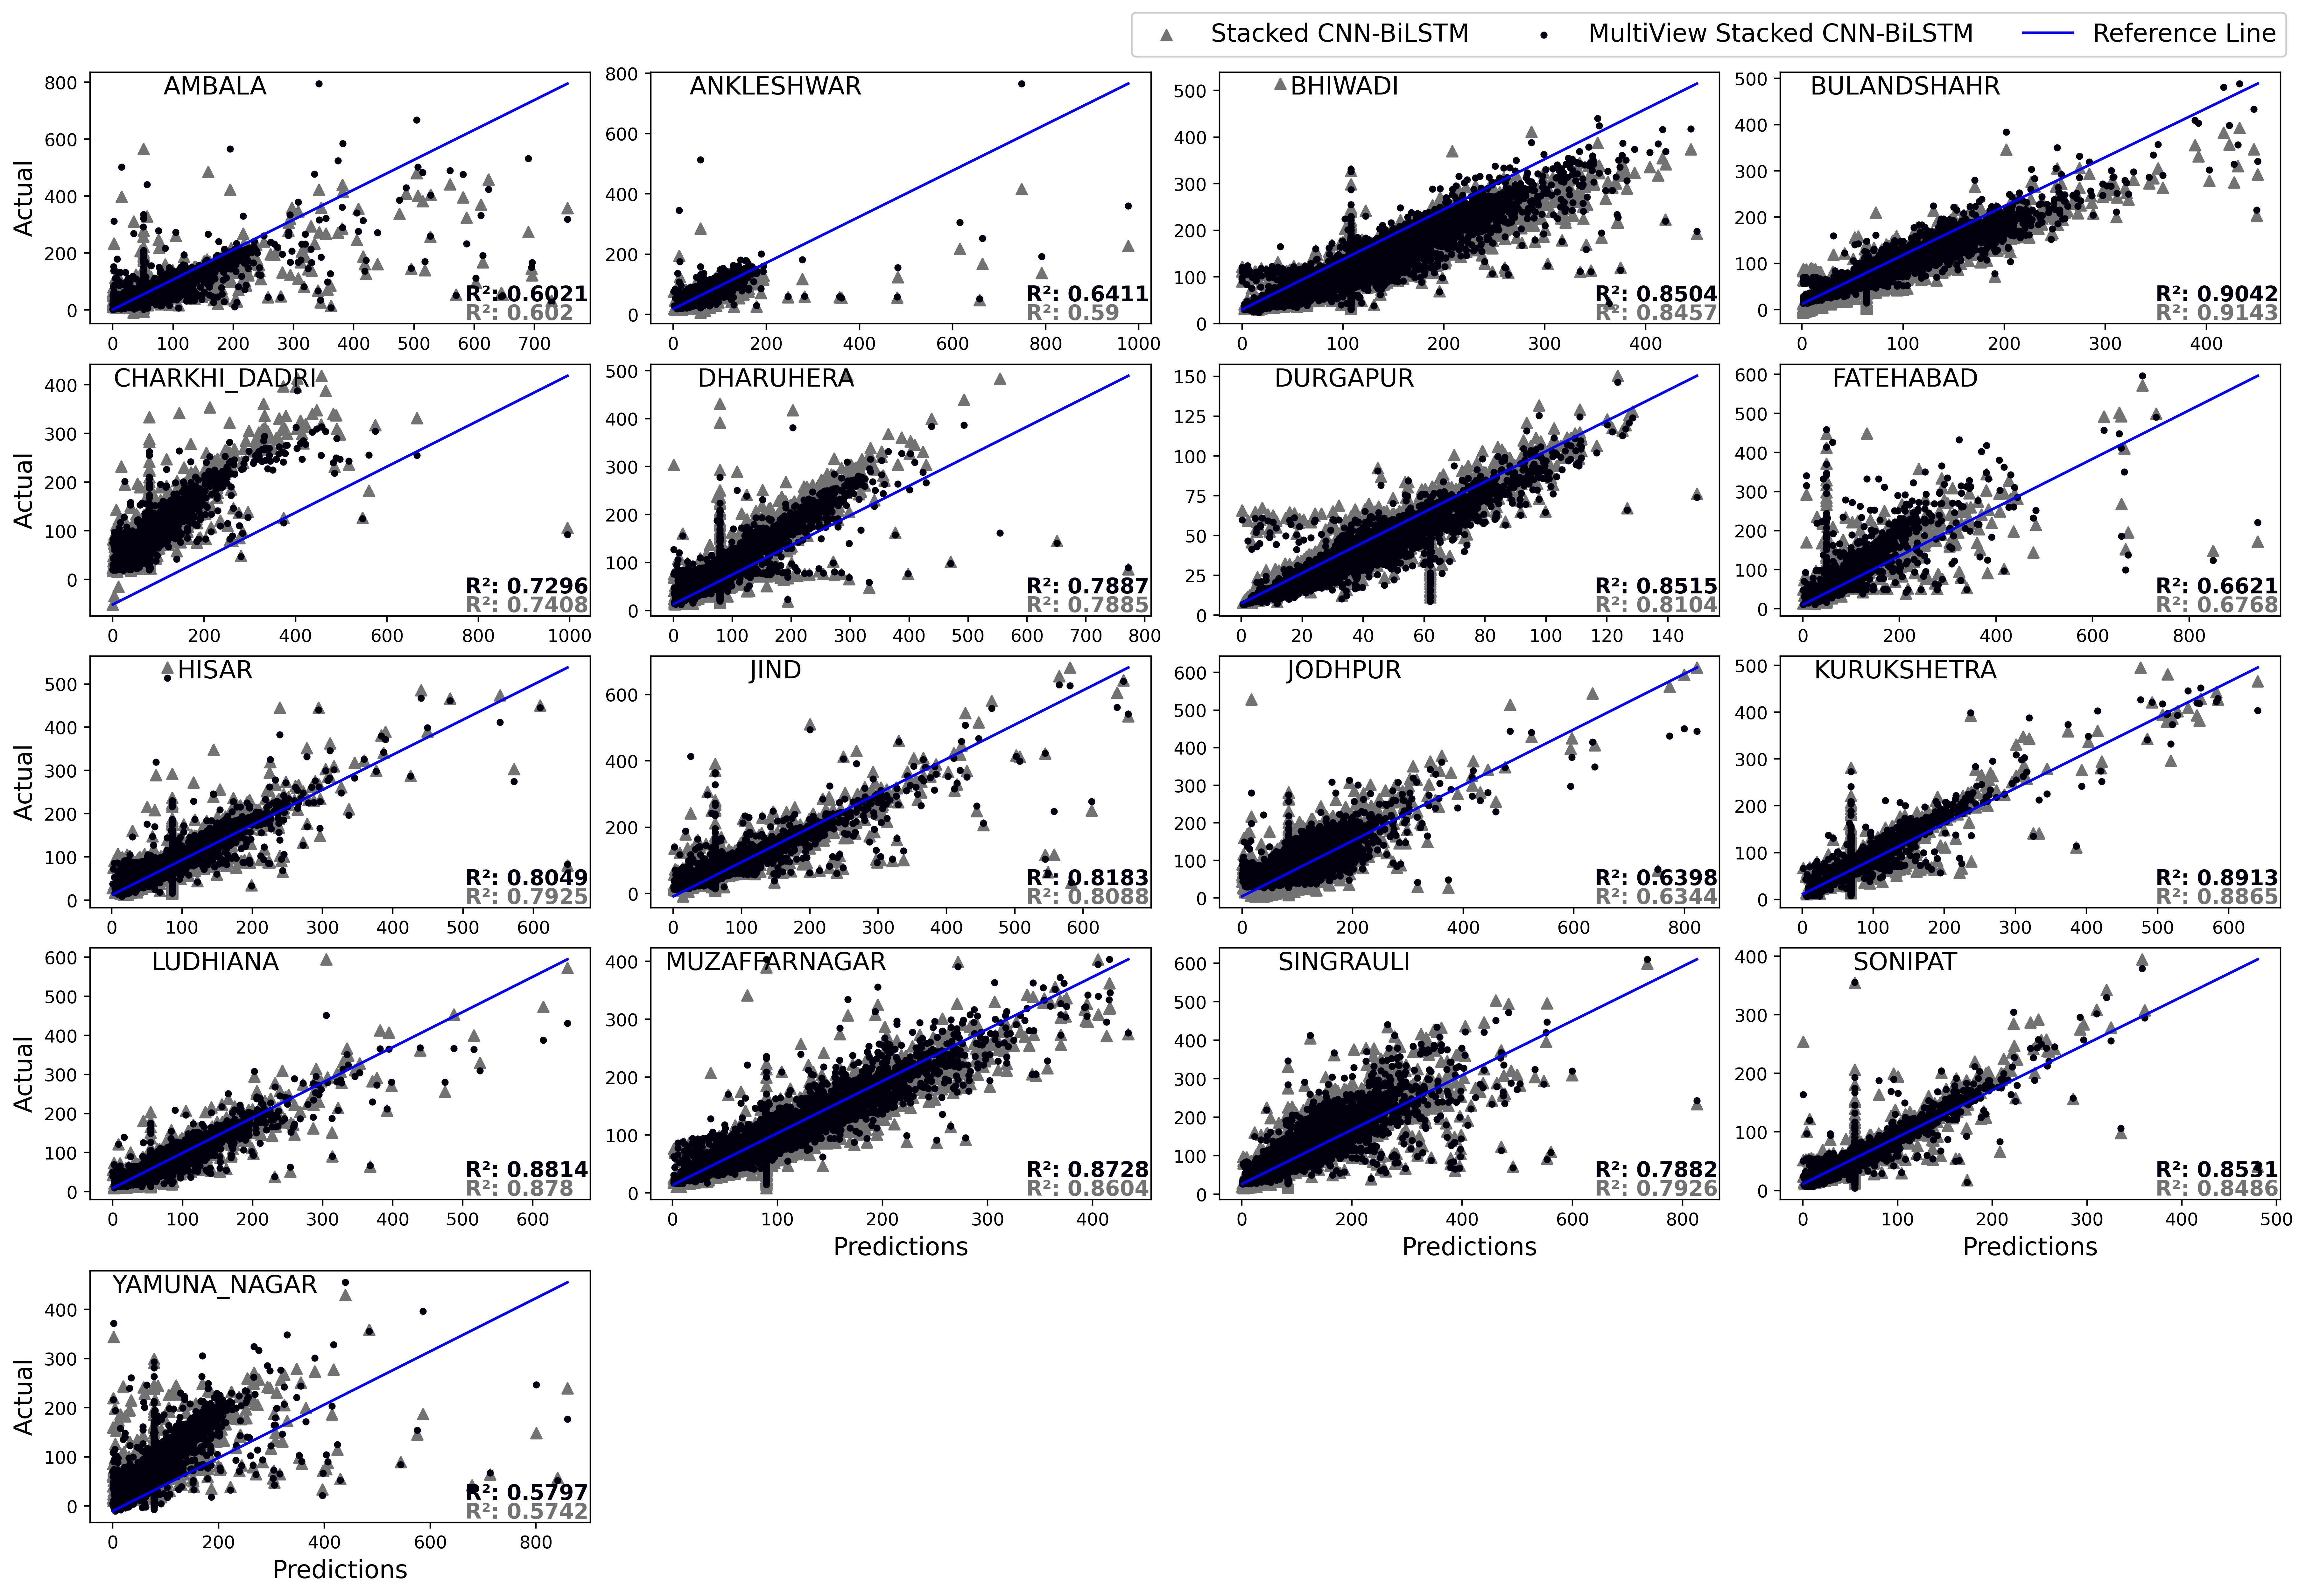
\includegraphics[scale=0.35]{Scatter_plot}
	  \caption{Correlation of Actual values and Predictions of proposed models $($Stacked CNN-BiLSTM and MvS CNN-BiLSTM $)$ using Scatter plot.}\label{Scatter}
\end{figure}
The \Cref{Scatter} contains 17 subplots,  each displaying a scatter plot for multiple datasets,  and compares the grey Stacked CNN-BiLSTM model with the black Proposed MvS CNN-BiLSTM model. The plot includes a blue reference line representing the optimal scenario in which predicted and actual values are aligned. Additionally,  each subplot displays two $R^2$ values corresponding to the grey and black superimposed plots. A heightened $R^2$ value suggests a more powerful correlation between anticipated and actual values,  making it a valuable statistical gauge of fitness in provided Figure; there are two potential interpretations:  If the grey Stacked CNN-BiLSTM has a more excellent $R^2$ value than the black Proposed MvS CNN-BiLSTM,  The analysis shows that the grey model had superior accuracy and a more resilient correlation between projected and actual values than the black model,  leading to a superior overall fit. The same $R^2$ value of the black Proposed MvS CNN-BiLSTM and the grey Stacked CNN-BiLSTM makes it irrelevant which model performed better in predicting actual values and has a similar goodness-of-fit and correlation with actual values. Based on the information you provided,  it appears that for the \Cref{Scatter} Singrauli,  Fatehabad,  Charkhi\_Dadri,  and Bulandshahr,  the grey Stacked CNN-BiLSTM model has higher $R^2$ values compared to the black Proposed MvS CNN-BiLSTM model. However,  you mentioned that the $R^2$ values for the black model are very close to the grey model. In this case,  since the $R^2$ values for the black model are very close to the grey model,  it suggests that both models have similar predictive performance for those datasets. The difference in their $R^2$ values might be slight,  indicating that they are both relatively accurate in predicting the actual values. It has concluded that the association of multi-view leading with stacked CNN-BiLSTM is performing better than the stacked CNN-BiLSTM along with the traditional model over various measures.


\begin{table}[!htp]
  \caption{Overall average of RMSE and MAPE ranking of traditional models and proposed model (MvS CNN-BiLSTM).}
  \centering
  \begin{tabular}{lccc}
  \hline
  Algorithm&RMSE\_Ranking&MAPE\_Ranking&Average\_Ranking\\\hline
  BiLSTM&3.7059&3.4706&3.58825\\
  CNN&4.8235&4.1765&4.5\\
  GRU&3.1765&3.7647&3.4706\\
  LSTM&3.8235&3.8824&3.85295\\
  RNN&3.7059&4.7059&4.2059\\
  \textbf{MvS CNN-BiLSTM}&\textbf{1.7647}&\textbf{1}&\textbf{1.38235} \\\hline
\end{tabular}
\label{AVG RANK}
  \end{table}



  \begin{figure*}[h!]
    \centering
    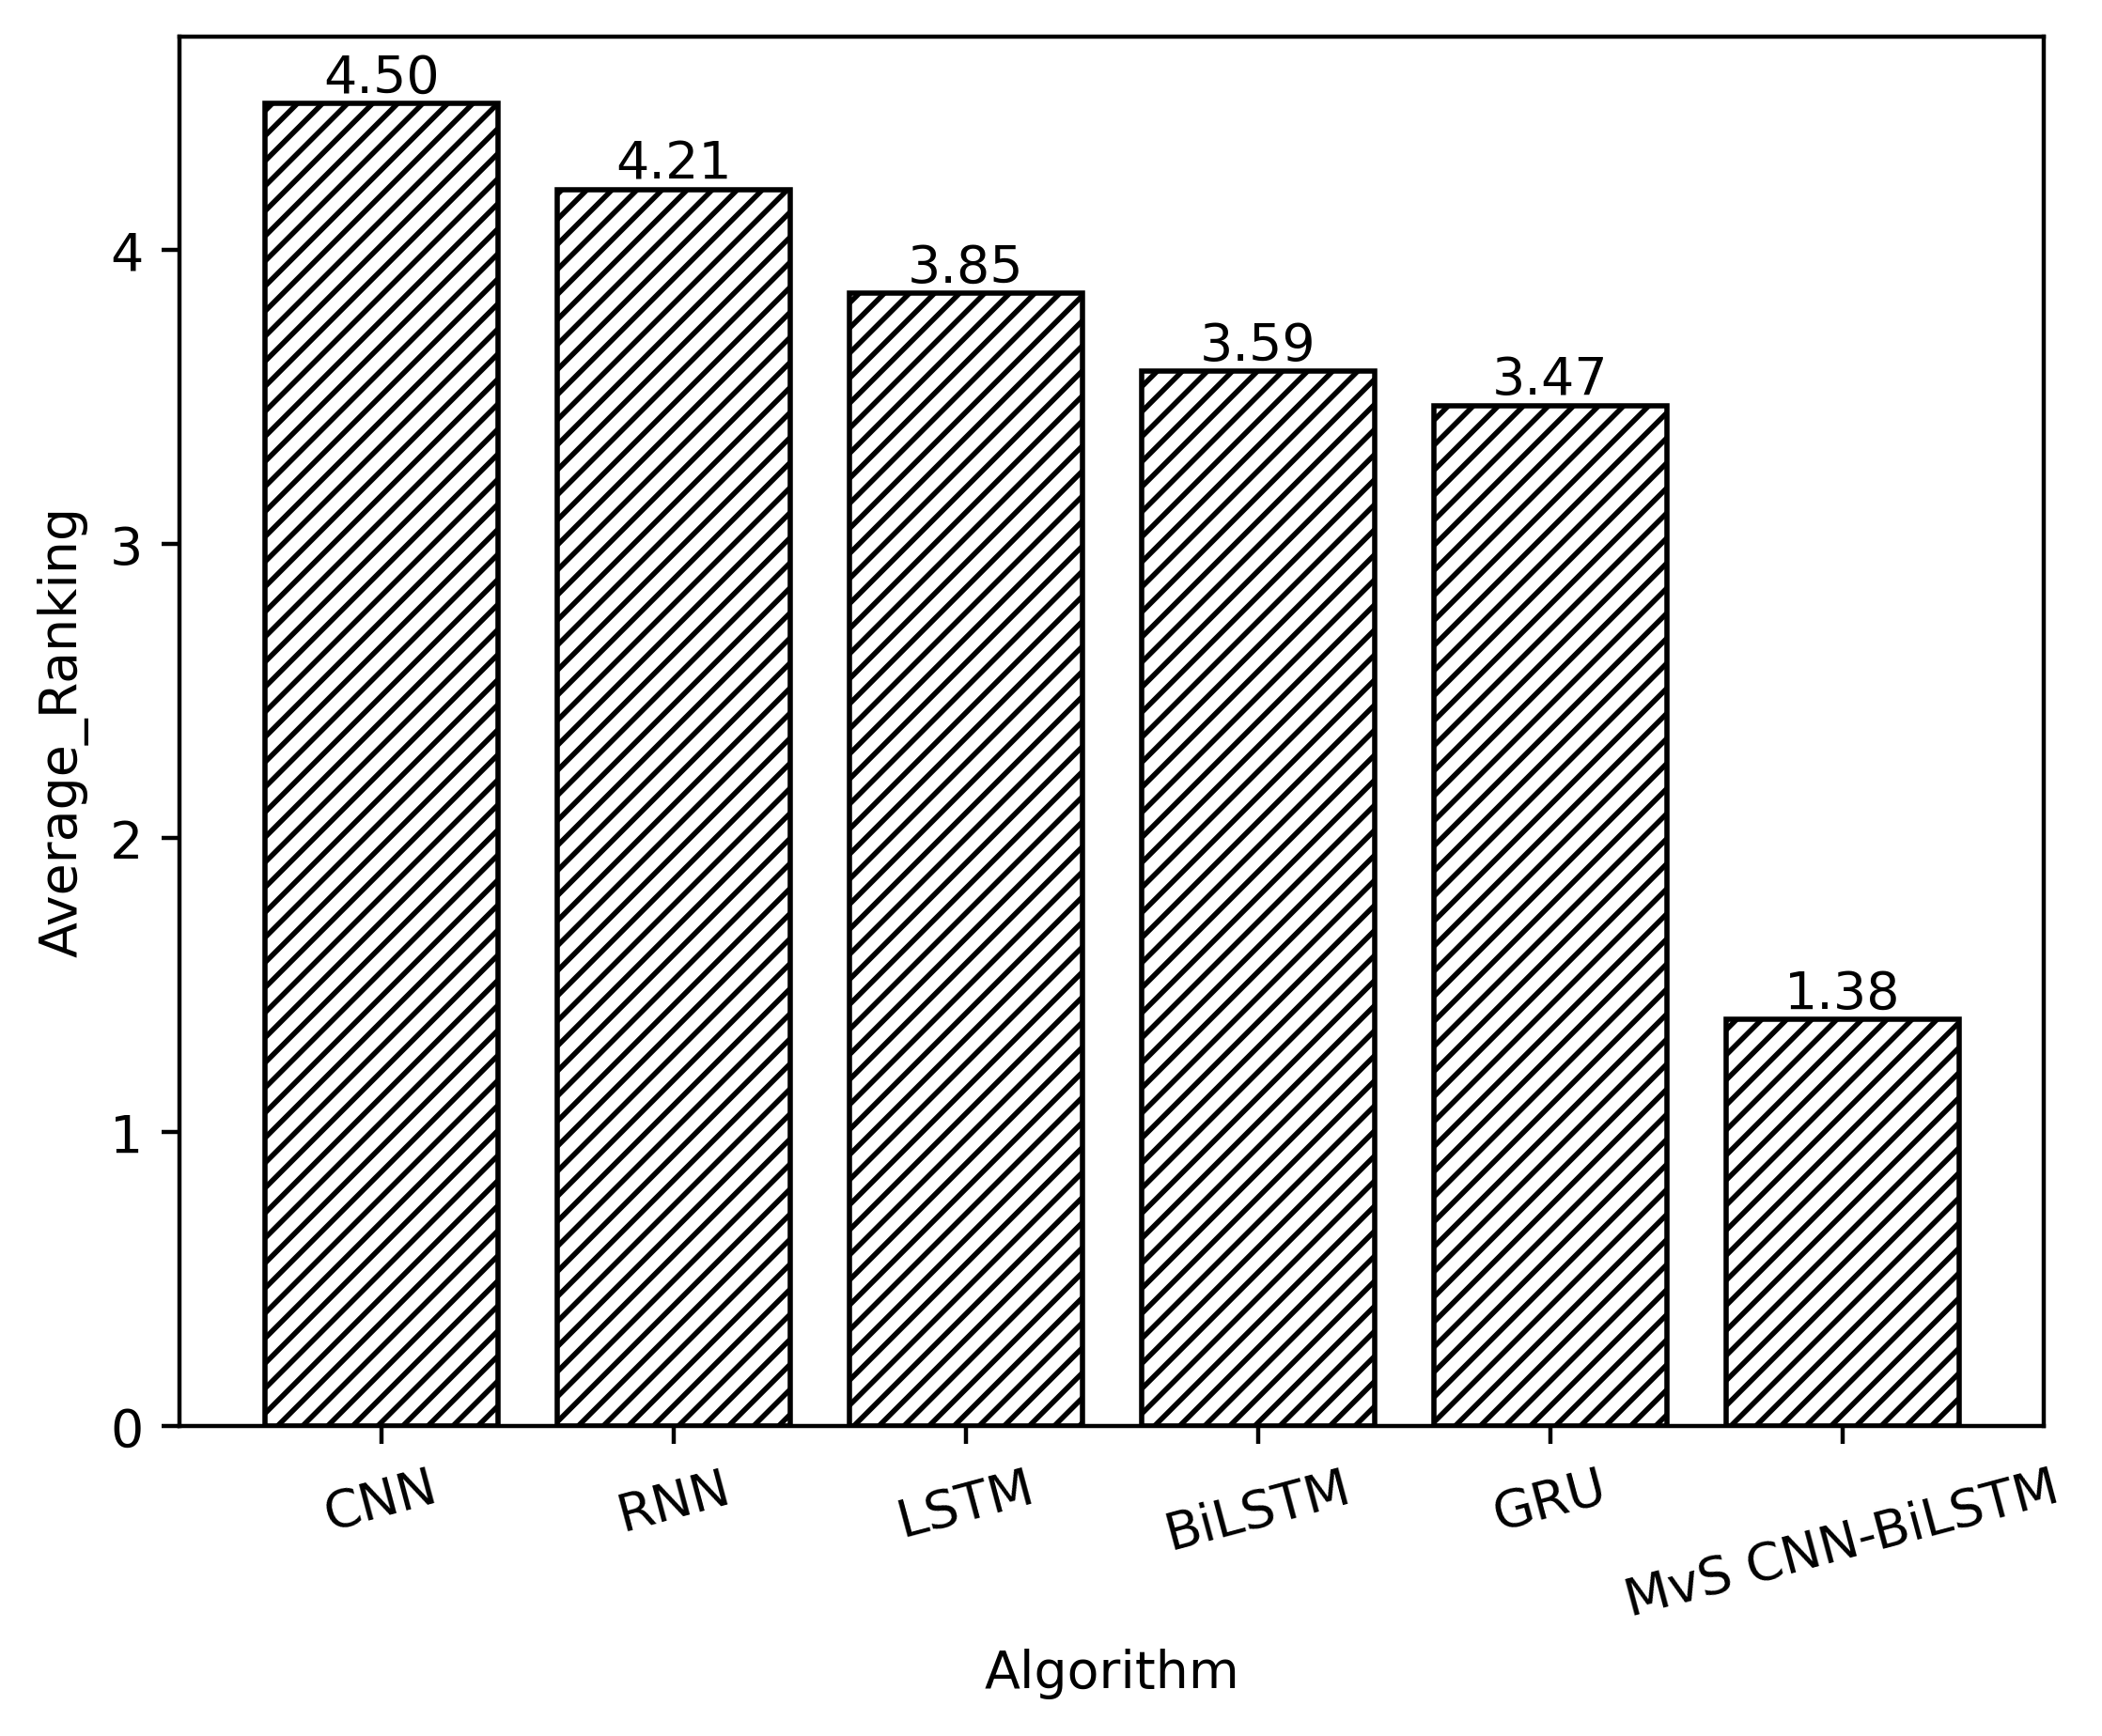
\includegraphics[scale=0.7]{avg_Rank_plot}
    \caption{Overall average Friedman ranking of traditional models and proposed MvS CNN-BiLSTM model.}
    \label{avg_Rank_plot}
  \end{figure*}
  In \Cref{AVG RANK},  the mean rankings of various algorithms are presented according to their performance on two performance metrics,  namely RMSE and MAPE. The table also includes an additional column for the average ranking across both metrics. The initial column suggests the average positions of each formula based on their RMSE performance. In contrast, the second column displays the average positions of each formula based on their MAPE performance. The third column signifies the mean rank of each algorithm,  factoring in performance on both metrics and providing a comprehensive measure of performance. In \Cref{AVG RANK} show average ranking on both performance measures and concluded the best algorithm. The underperformance of conventional deep learning structures such as BiLSTM,  CNN,  GRU,  LSTM,  and RNN,  despite their higher ranking on average,  is a surprising observation compared to the MvS CNN-BiLSTM method. Thus,  according to \Cref{avg_Rank_plot}, the mean ranking over the two performance metrics,  the MvS CNN-BiLSTM algorithm is regarded as the optimal algorithm out of all the models. The bar graph provided is illegible and cannot be used to support the previous analysis,  showing that the MvS CNN-BiLSTM algorithm has no ranking or comparison to the traditional deep learning models (BiLSTM,  CNN,  GRU,  LSTM,  and RNN) on average for the given task. The CNN and RNN algorithms were rated the worst on average,  suggesting their performance was not as great as other models.





\section{Conclusions}
Our findings from analysing the forecasting of $PM_{2.5}$ levels in Indian cities using deep learning techniques have led us to several conclusions. The suggested MvS CNN-BiLSTM methods have been proven effective for predicting Indian city $PM_{2.5}$ levels. The implementation of intricate training models has furnished optimistic findings,  implying that they boast the potential to augment air quality projections considerably. It should be noted,  nonetheless,  that these models' performance relies on the specific city and season. Some locations may produce more precise forecasts than others,  highlighting the importance of customising the models to different geographical regions and seasons.


\section*{CRediT authorship contribution statement}

\section*{Data availability}
Data will be available on \href{https: //app.cpcbccr.com/ccr/#/caaqm-dashboard-all/caaqm-landing}{CPCB(India)} Webportel.The \href{https: //www.cpcb.nic.in/}{Central Pollution Control Board (CPCB) } in India maintains a web portal that offers access to various environmental datasets,  including air and water quality,  emission inventories,  and pollution monitoring data,  aimed at promoting environmental awareness and research in the country.
\section*{Acknowledgments}
We extend our heartfelt appreciation to the Central Pollution Control Board (CPCB),  India,  for generously providing invaluable environmental data,  which significantly enhanced our research and played a pivotal role in completing this study.
\label{}

% Numbered list
% Use the style of numbering in square brackets.
% If nothing is used, the default style will be taken.
%\begin{enumerate}[a)%\item 
%\item 
%\item 
%\end{enumerate}  

% Unnumbered list
%\begin{itemize}
%\item 
%\item 
%\item 
%\end{itemize}  

% Description list
%\begin{description}
%\item[]
%\item[] 
%\item[] 
%\end{description}  


\begin{comment}

\begin{table}[<options>]
\caption{}\label{tbl1}
\begin{tabular*}{\tblwidth}{@{}LL@{}}
\toprule
 & \\ % Table header row
\midrule
 & \\
 & \\
 & \\
 & \\
\bottomrule
\end{tabular*}
\end{table}



\end{comment}
% Uncomment and use as the case may be
%\begin{theorem} 
%\end{theorem}

% Uncomment and use as the case may be
%\begin{lemma} 
%\end{lemma}

%% The Appendices part is started with the command \appendix;
%% appendix sections are then done as normal sections
%% \appendix




\label{}

% To print the credit authorship contribution details
\printcredits

%% Loading bibliography style file
%\bibliographystyle{model1-num-names}
\bibliographystyle{cas-model2-names}

% Loading bibliography database
\bibliography{ref}

% Biography
\bio{}
% Here goes the biography details.
\endbio

%\bio{pic1}
% Here goes the biography details.
\endbio

\end{document}